%
\chapter{Sequências e Séries de Funções}

\section{Sequência de Funções: Converg\^encia  Pontual}
%%%
O tipo mais natural de converg\^encia para uma sucess\ao\ de fun\coes\ provavelmente \'e pontual 
(ou simples) converg\^encia, definido como segue.

\begin{defic}{Convergência Pontual de Sequência de Funções}{} 
Uma \seq\ de funções de $\mathbb{R}^p$ em
$\mathbb{R}^m$ é uma função cujo domínio é o conjunto dos interios
positivos e cuja imagem é um conjunto de funções de $\mathbb{R}^p$
em $\mathbb{R}^m$. A \seq\ de funções de $\mathbb{R}^p$ em
$\mathbb{R}^m$ é representada por $\{f_n\}$.

Para cada ponto $x$ do domínio de todos os termos da \seq\ de
funções $\{f_n\}$, existe uma \seq\ de pontos $\{f_n(x)\}$. Se
$\{f_n(x)\}$ converge para cada ponto $x$ de um conjunto
$\mathcal{E}$ e fazemos
\begin{equation*}
    f(x)=\lim_{n\to \infty}f_n(x),
\end{equation*}
então dizemos que $\{f_n\}$ \textbf{converge pontualmente}  a $f$
sobre $\mathcal{E}$.
\end{defic}

De forma equivalente em dimensões menores. Uma \seq\ $\{f_n\}$
onde cada elemento é uma função $f_n\colon I\subseteq
\mathbb{R}\to \mathbb{R}$, \textit{converge pontualmente em I} se
existe o limite
\begin{equation*}
  \lim_{n\to\infty}f_n(x_{0})
\end{equation*}
relativamente a cada $x_{0}$ de $I$.


\begin{exer} 
Seja $f_n(x) =x^n,\quad 0\leq x\leq 1$, $n= 1,\; 2,\;  3,\ldots$
Verifique a convergência pontual.
\end{exer}

\solo Para $0\leq x_{_{0}}<1$ temos
\begin{equation*}
  \lim_{n\to\infty} f_n(x_{_{0}}) = \lim_{n\to\infty} x_{_{0}}^n=0,
\end{equation*}
ao passo que, quando $x =1$, $\dst{\lim_{n\to\infty}f_n(1) = 1}$.

A sequência dada, portanto, converge pontualmente no intervalo $0
\leq  x \leq 1$ para a função
\begin{equation*}
  f(x) =
    \begin{cases}
      0 & \quad \text{ se } \quad 0\leq x < 1 \\[2ex]
      1 & \quad \text{ se }\quad x=1
    \end{cases}
\end{equation*}
veja o lado esquerdo da Figura~\ref{fig-1116-5}.
\begin{figure}[H]
\centering
\includegraphics[width=0.6\textwidth]{fig-1116-5.eps}
\caption{Convergência Pontual}
\label{fig-1116-5}
\end{figure}

Observemos que, enquanto cada uma das $f_n$ é contínua no
intervalo inteiro $0 \leq x \leq 1$, a função limite $f$ não é
contínua neste intervalo (ela é descontínua em $x = 1$).

Em no caso geral a \seq\ $\{x^n\}$ para $x\in \mathbb{R}$ converge
para zero se $x\in ]-1, \; 1[$, converge para um se $x=1$, e diverge
se $x\in ]-\infty, \; -1]\cup ]1, \; \infty[$. Portanto a \seq\ converge
pontualmente sobre $\mathcal{E}=]-1,\; 1]$ para a função $f$ onde
\begin{equation*}
  f(x) =
    \begin{cases}
      0 & \text{ se } \quad -1< x < 1 \\[2ex]
      1 & \text{ se } \quad x=1
    \end{cases}
\end{equation*}

Observamos que cada termos da \seq\ de funções é uma função
contínua, a função limite $f$ não é contínua.\qed

Mesmo que a convergência uniforme é suficiente para garantir que o
limite de uma \seq\ de funções contínuas é contínua, não é uma
condição necessária para este resultado. No seguinte exemplo, a
\seq\ de funções contínuas não converge uniformemente e mesmo
assim a função limite $f$ é contínua

\begin{exer}\label{ex1116-2}
Seja a \seq\ $\{f_k\}$ onde cada função esta definida em $0\leq x
\leq 2$, onde
\begin{equation*}
    f_1(x)=k^2,\quad 0\le x\le 2
\end{equation*}
e para $k\ge 2$ seja
\begin{equation*}
  f_k(x) =
    \begin{cases}
      k^3x & \text{ se}, \quad 0\le x \le 1/k \\[2ex]
      2k^2-k^3x & \text{ se},\quad 1/k<x\le 2/k\\[2ex]
      0 &\text{ se}, \quad  2/k<x\le 2
    \end{cases}
\end{equation*}
cujo gráfico esta indicado no lado direito da
Figura~\ref{fig-1116-5}. Discutir a convergência pontual.
\end{exer}

\solo Evidentemente, $f_k(0)= 0$ para todo $k$, donde
$\dst{\lim_{n\to\infty}f_k(0) = 0}$. Mais ainda, se $0 < x_o\leq
2$, então existe algum valor de $k$, digamos $N$, tal que $2/N <
x_o$ e, assim, $f_k(x_o) = 0$ para todo $k \geq N(\varepsilon)$.

Portanto, $\dst{\lim_{k\to\infty} f_k(x_o) = 0}$, e concluímos que
$\{f_k(x)\}$ converge pontualmente para a função identicamente
nula no intervalo $0\leq x \leq 2$ e portanto contínua. Porém a
convergência não é uniforme, pois para qualquer $k$ se $x=1/k$,
então $|f_k(x)-f(x)|=k^2$.

Desta vez, a sequência de funções contínuas converge para um
\textit{limite contínuo}. Apesar disto, as funções $f_k$, não
importa a que distância elas estejam na sequência, podem diferir,
por grande margem, da função limite $f(x)\equiv 0$. Por
conseguinte, os elementos da sequência não são ``aproximações"\;
do limite da sequência no sentido que se espera do termo. E as
integrais dos termos da sequência refletem êste comportamento
peculiar, deixando de tender para a integral da função limite
$f(x)$.

De fato, $\dst{\int_0^2f(x)dx = 0}$, enquanto que
\begin{equation*}
  \int_0^2f_k(x)dx =\frac{1}{2}\cdot\frac{2}{k}\cdot k^2=k
\end{equation*}
e tendem para infinito, não-zero, quando $k$ vai ao infinito.\hfill \(\lozenge\)

A fim de eliminar esta espécie de comportamento, introduzamos
agora um tipo de convergência mais forte, denominada
\textit{convergência uniforme}.

%%%%
\section{Sequência de Funções: Convergência Uniforme}
%%%%

Muitas das fun\c c\~oes que n\'os estudamos serão definidas por
meio de sucess\oes\ infinitas ou s\'eries. Para estudar tais
fun\coes\ precisamos entender o conceito de converg\^encia
uniforme de uma sucess\ao\ ou s\'erie de  fun\coes\ (cont\ii
nuas). Para lidar efetivamente com situa\coes\ concretas e
exemplos, nós também consideraremos v\'arios importantes testes de
converg\^encia uniforme.

Talvez o teste mais \'util em exemplos particulares s\ao\ o
M-teste de Weierstrass para s\'eries. Outro teste \'e o Critério
de Cauchy que \'e principalmente de uso te\'orico. N\'os tamb\'em
inclu\ii mos os testes mais refinados de Dirichlet e Abel.

Em conexão  com a converg\^encia uniforme introduzimos um espa\co\
cujos pontos s\ao\ fun\coes.\ Neste espa\co\ n\'os introduzimos
uma norma e mostramos  que a converg\^encia nesta esta norma \'e
precisamente a converg\^encia uniforme. O espa\co\ é completo no
sentido que sucess\oes\ de Cauchy convergem. Uma segunda
propriedade b\'asica deste espaço, chamada de teorema de
Arzela-Ascoli, estabelece a compacidade de um subconjunto (no
sentido de possuir a propriedade de Bolzano-Weierstrass). Outro
resultado importante, chamado de teorema o Stone-Weierstrass
também é provado. Este teorema permite  aproximar fun\coes\
cont\ii nuas através de polin\^omios, ou por fun\coes\ de outras
classes apropriadas. Finalmente, algumas aplica\coes\ desta
maquinaria s\ao\ fornecidas para\ equa\coes\  diferenciais e
integrais.

\begin{defic}{}{} Uma sequência de funções $\{f_n\}$ \textbf{converge
uniformemente} para a função $f$ sobre o conjunto $\mathcal{E}=[a,
b]$, se para todo $\varepsilon > 0$ existe um número inteiro positivo
$N= N(\varepsilon) \in \mathbb{N}$, dependente de $\varepsilon$ mas não 
de $x$, tal que para todo $x\in \mathcal{E}$
\begin{equation*}
  |f_n(x) - f(x)|< \varepsilon\quad \text{ sempre que }\quad  n>
  N(\varepsilon).
\end{equation*}
\end{defic}

É claro, evidentemente, que, se $\{f_n\}$ converge uniformemente
para $f$ em $a\leq x\leq b$, então ela também converge
\textit{pontualmente} para $f$ neste intervalo. Porém a
convergência pontual de $\{f_n\}$ para $f$ sobre $\mathcal{E}$ não
implica a convergência uniforme da \seq\ para $f$ sobre
$\mathcal{E}$.

Realmente podemos alcançar a convergência uniforme
a partir da convergência pontual se e somente se para cada
$\varepsilon>0$ existe um conjunto de números $\{N(x)\colon x\in
\mathcal{E}\}$ superiormente limitado (acotado). Se $\{f_n\}$ converge
pontualmente para $f$ sobre $\mathcal{E}$ e $N$ é uma cota
superior (majorante) do conjunto $\{N(x)\colon x\in \mathcal{E}\}$, então para
todo $x\in \mathcal{E}$
\begin{equation*}
    |f_n(x)-f(x)|<\varepsilon\quad\text{sempre que }\quad n>N.
\end{equation*}

Assim, $\{f_n\}$ é uniformemente convergente para $f$ sobre
$\mathcal{E}$. Além disso, se $\{f_n\}$ é uniformemente
convergente a $f$ sobre $\mathcal{E}$ e $N$ corresponde para
$\varepsilon>0$, então para cada $x\in \mathcal{E}$ podemos tomar
$N(x)=N$ e o conjunto $\{N(x)\colon x\in \mathcal{E}\}$ ficara
(acotado) limitado superiormente por $N$.

No caso, da convergência uniforme, pode-se escolher $n$ de
modo tal que
\[
f(x) -\varepsilon<f_n(x)<f(x) +\varepsilon
\]
para cada $x$ no intervalo $a\leq x \leq b$. Portanto, $f_n$ é uma
aproximação de $f$ com diferença inferior a $\varepsilon$, no
intervalo todo, como o mostra a Figura~\ref{fig-1116-7}.
\begin{figure}[H]
\centering
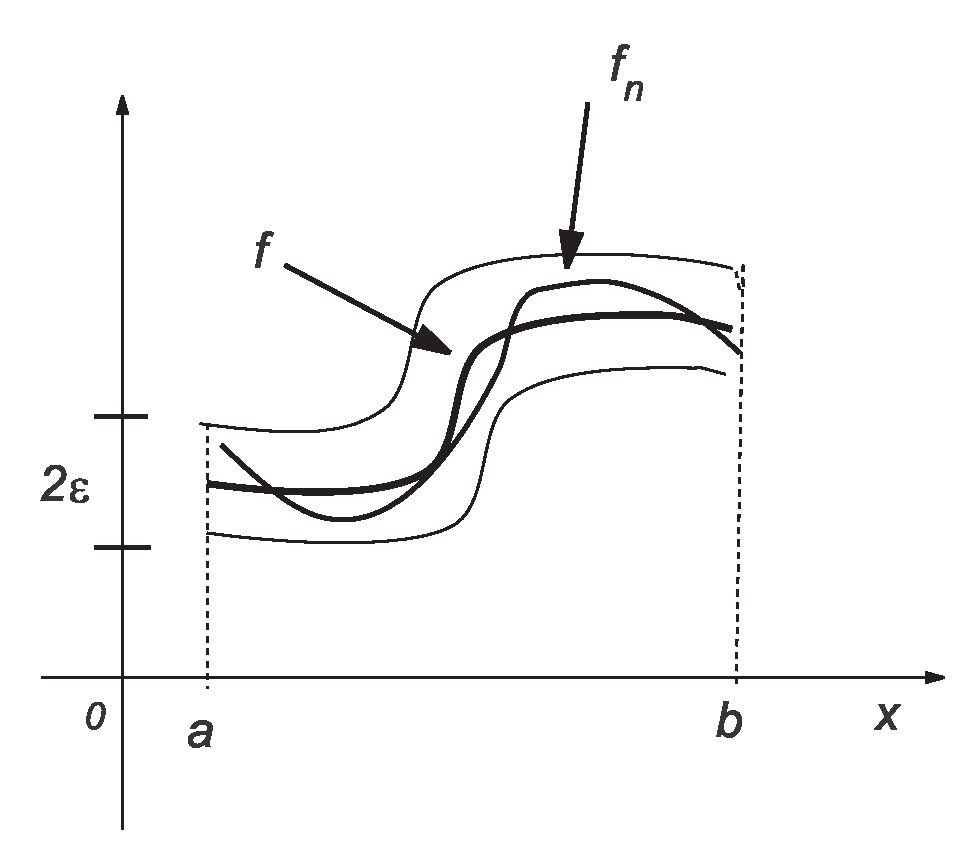
\includegraphics[width=0.45\textwidth]{fig-1116-7.eps}
\caption{Convergência Uniforme}
\label{fig-1116-7}
\end{figure}

Observamos, no Exemplo~\ref{ex1116-2}, que no caso de convergência
pontual nenhum dos termos da sequência é, necessáriamente, uma
aproximação da função limite, nesse sentido.

\begin{exer}
Escrever cuidadosamente as defini\coes\ de converg\^encia pontual
(ou simples) e converg\^encia uniforme. Com as defini\coes\
anteriores verifique a seguinte implicação,
\begin{center}
Converg\^encia uniforme $\ent$ Converg\^encia Pontual
\end{center}
\end{exer}

\solo A \seq\ de fun\coes\ $u_n\colon I\subset \R\to \R$ converge
pontualmente para a $u\colon I\subset \R\to \R $ ou $(u_n\to u)$
sobre o conjunto $I\subset \R$ se para cada $\mathbf{\varepsilon}$
e para cada $x\in I$ existe um n\'umero, $N=
N(x,\mathbf{\varepsilon})$ tal que,
\begin{equation*}
|u_n(x)-u(x)|<\mathbf{\varepsilon}\quad \text{ sempre que } \quad n>N.
\end{equation*}


Definimos a converg\^encia uniforme: a \seq\
de fun\coes\ $u_n\colon I\subset \R\to \R$ converge uniformemente
a $u\colon I\subset \R\to \R$ ($u_n\rightrightarrows u$) sobre o
conjunto $I\subset \R$ se para cada $\varepsilon$ existe um
n\'umero, $N= N(\mathbf{\varepsilon})$ tal que se para todo $x\in
I$,
\begin{equation*}
|u_n(x)-u(x)|<\mathbf{\varepsilon}\quad \text{ sempre que } \quad n>N.
\end{equation*}

Observamos que $u_n \uni u (\uni)$ implica $u_n \to u$. Pois se funciona para todo $x\in I$, em particular para cada $x\in I$, 
e para $\mathbf{\varepsilon}>0$ dado,  temos $N=N(x, \mathbf{\varepsilon})$ tal que
\begin{equation*}
|u_n(x)-u(x)|<\mathbf{\varepsilon}\quad \text{sempre que}\quad n>N.
\end{equation*}

Assim obtemos a converg\^encia simples, $u_n\to u$. \qed

No contexto da convergência uniforme temos que:
\begin{equation*}
    \text{Limite uniforme} = \text{Limite pontual}
\end{equation*}

Lembremos também que convergência pontual não implica convergência uniforme como será ilustrado no seguinte contra-exemplo;

\begin{exer}
Seja a seguinte \seq de funções $\{f_n\}$ aonde cada termo é
\begin{equation*}
    f_n(x)=\frac{nx}{1+(nx)^2},\qquad x\in \mathbb{R}.
\end{equation*}

Mostre que não converge uniformemente em qualquer intervalo
$[a,b]$ tendo o zero como seu ponto interior.
\end{exer}

\solo Como podemos ver, aplicando resultados de convergência
simples, a \seq $\{f_n\}$ converge pontualmente com limite pontual
$f$ tal que
\begin{equation*}
    f(x)=0,\qquad x\in \mathbb{R}.
\end{equation*}

A seguir mostramos que a convergência não é uniforme em qualquer
intervalo $[a,b]$ que contenha o ponto zero como ponto interior.

Suponhamos que a convergência seja uniforme sobre $[a,b]$ de forma
que o limite pontual seja também limite uniforme.

Seja $\varepsilon>0$ dado. Então existe $N$ tal que para todo $n>
N$ e para todo $x\in [a,b]$,
\begin{equation*}
    \left|\frac{nx}{1+(nx)^2}-0 \right|<\varepsilon.
\end{equation*}

Tomar $\varepsilon=1/8$. Também existe um $k\in \mathbb{Z}$  tal
que
\begin{equation*}
    k> N\quad \text{ e }\quad 1/k\in [a,b].
\end{equation*}

Tomando $n=k$ e $x=1/k$, temos
\begin{equation*}
    \frac{nx}{1+(nx)^2}=\frac{1}{2}
\end{equation*}
resultado que não é menor que $1/8$.

Assim chegamos a uma contradição e vemos que a convergência não é
uniforme em qualquer intervalo que contenha o ponto zero como
ponto interior, mesmo que nele exista a convergência clásica ou pontual. \hfill \(\lozenge\)

\begin{theoc}{Critério de Cauchy}{}
A condição necessária e suficiente para
que uma \seq de funções $\{f_n\}$ definidas em $I$ seja
\textit{uniformemente convergente} é que para cada
$\varepsilon>0$, existe $N=N(\varepsilon)\in \mathbb{N}$ tal que
\begin{equation*}
n \geq N,\quad \forall\; p\ge 0,\quad \forall\; x\in I,\quad \text{implica,}
\quad   |f_{n+p}(x)-f_n(x)|<\varepsilon.
\end{equation*}
\end{theoc}

\prova (A condição Necessária \((\Rightarrow)\)) Seja a \seq $\{f_n\}$
uniformemente convergente com $f$ como seu limite uniforme.

Seja $\varepsilon>0$ fornecido. Então existe $N$ tal que se $n\ge
N$ e para todo $x\in I$,
\begin{equation*}
    |f_n(x)-f(x)|<\varepsilon/2.
\end{equation*}

Também como $n> N$ e para todo $p\ge 0$ e para todo $x\in I$,
\begin{equation*}
    |f_{n+p}(x)-f(x)|<\varepsilon/2,
\end{equation*}
disto segue que para $n> N$, para todo $p\ge 0$ e para todo $x\in
I$,
\begin{align*}
|f_{n+p}(x)-f_n(x)|&=|f_{n+p}(x)-f(x)+f(x)-f_n(x)|\\[2ex]
&\le |f_{n+p}(x)-f(x)|+|f(x)-f_n(x)|<\varepsilon.
\end{align*}

(A condição Suficiente \((\Leftarrow )\))
Pelo princípio de
convergência de Cauchy, segue que a \seq converge pontualmente.
Todo o que temos a mostrar é que convergência seja uniforme.
Considere $f$ o limite pontual da \seq $\{f_n\}$. Seja
$\varepsilon>0$ dado, então existe $N$ tal que para $n> N$, para
todo $p\ge 0$ e para todo $x\in I$,
\begin{equation*}
|f_{n+p}(x)-f_n(x)|< \varepsilon/2\quad\textrm{ implica }\quad
f_n(x)-\varepsilon/2<f_{n+p}(x)<f_n(x)+\varepsilon/2.
\end{equation*}

Mantendo $n$ fixo e fazendo $p$ tender para o infinito, vemos que
para $n> N$ e para todo $x\in I$,
\begin{equation*}
    f_n(x)-\varepsilon/2\le f(x)\le f_n(x)+\varepsilon/2\quad
    \textrm{ implica }\quad
 |f_n(x)-f(x)|\le\varepsilon/2<\varepsilon.
\end{equation*}

Assim a convergência é uniforme. \hfill \(\square\)

\begin{exer}
Prove que a \seq\ de funções $\{x^n\}$ convergente uniformemente
sobre $[-a,\; a]$, onde $0<a<1$.
\end{exer}

\solo Para cada $x\in [-a,\; a]$ temos
\begin{equation*}
    \lim_{n\to\infty} x^n=0\quad \text{e }\quad |x^n-0|=|x^n|\leq
    a^n.
\end{equation*}

Para qualquer $\varepsilon>0$, temos que $a^n<\varepsilon$ sempre
que $n>\ln(\varepsilon)/\ln\, a$.

Assim, se escolhemos $N=ln(\varepsilon)/ln\, a$, temos que para
qualquer $x\in [-a,\; a]$,
\begin{equation*}
    |x^n-0|<\varepsilon\quad \text{sempre que }\quad n>N.
\end{equation*}

O que mostra que $\{x^n\}$ converge uniformemente para zero sobre
o conjunto $[-a, \; a]$. \hfill \(\lozenge\)

\begin{exer}
Prove que a \seq\ de funções $\{x^n\}$ não converge uniformemente
 sobre $]-1, \; 1[$.
\end{exer}

\solo Tomar um $\varepsilon$ qualquer tal que $0<\varepsilon<1$.
Para cada $x\in ]-1,1[$ temos que
\begin{equation*}
    \lim_{n\to\infty}x^n=0,
\end{equation*}
e portanto existe um número $N(\varepsilon,x)$ tal que
\begin{equation*}
    |x^n-0|=|x^n|<\varepsilon,\quad \text{sempre que}\quad n>N(\varepsilon, x).
\end{equation*}

Como a desigualdade $|x|^n=|x^n|<\varepsilon$, então se e somente se $n>\ln
\varepsilon/\ln |x|$ e como
\begin{equation*}
    \lim_{x\to 1^{-}}\frac{\ln \varepsilon}{\ln x}=\infty,
\end{equation*}
o conjunto $\{N(x)\colon x\in \mathcal{E}=]-1,1[\}$ não pode ser
acotado superiormente. Isto é, não pode existir nenhum número $N$
tal que para todo $x\in ]-1,1[$
\begin{equation*}
    |x^n-0|<\varepsilon\quad \text{ sempre que }\quad n>N.
\end{equation*}

Obtemos assim o resultado desejado. \hfill \(\lozenge\)

Agora provaremos que uma \seq\ uniformemente convergente de
funções contínuas converge a uma função contínua.

\begin{exer}
Considere a \seq\  de fun\coes\  $\{u_n(x)\}_{n\geq 1}$ onde o n-ésimo termo tem a seguinte lei
de forma\c c\~ao;
$$
u_n(x)= x^n \quad \text{ onde, }\quad 0\leq x \leq 0,888.
$$
Mostrar que converge uniformemente.
\end{exer}

\solo  Vejamos que tem convergência pontual; por propriedade
anteriormente estudada, tem-se
$$
u_n(x)\to u(x)=0\quad \text{ para } \quad 0<x<1
$$

Para encontrar convergência uniforme tomamos esse limite $u(x)=0$
e aplicamos defini\cao;\ no intervalo $[0, 0,888]$, isto \'e, para
$\varepsilon>0$, devemos mostrar a exist\^encia do número
$N(\varepsilon)>0$. Sendo assim, fazemos os seguintes cálculos
\begin{equation}\label{marisa1}
|u_n(x)-u(x)|=|u_n(x)-0|=|u_n(x)|=|x^n|=|x|^n<(0,888)^n
\end{equation}

Utilizando a rela\cao\ \eqref{marisa1} e resolvendo a inequa\cao\
$(0,888)^n<\varepsilon$ para $n$ temos; $$ (0,888)^n<\varepsilon
\ent n\ln 0,888<\ln \varepsilon \ent n>\frac{\ln \varepsilon}{\ln
0,888}, \quad \text{ pois }\quad \ln 0,888 <0 $$ e assim podemos
tomar o número $N(\varepsilon)=\dst{\frac{\ln \varepsilon}{\ln
0,888}}$. \hfill \(\lozenge\)

\begin{exer}
 Considere a \seq\ de fun\coes, $\{u_n\}$ onde,
$$
\left\{\Bigl(x-\frac{2}{n} \Bigr)^2\right\}_{n\geq 1},\qquad 0\le x\le 1
$$

Fazer os cálculos correspondentes para verificar a sua
converg\^encia uniforme.
\end{exer}

\solo Desenvolvendo o quadrado para melhor cálculo da convergência
pontual;
$$
u_n(x)=x^2-\frac{4x}{n}+\frac{4}{n^2}\to x^2,
$$
para cada $x$ fixo. Escolhemos a fun\cao\ limite $u(x)=x^2$. Para mostrar
convergência uniforme, utilizamos a defini\cao,\ isto \'e para $\varepsilon>0$, devemos mostrar a
existência do número $N(\varepsilon)>0$. Sendo assim, fazemos os
seguintes cálculos;
\begin{equation}\label{marisa}
\begin{split}
  |u_n(x)-u(x)|=\left|-\frac{4x}{n}+\frac{4}{n^2}\right|&\leq
  \frac{4|x|}{n}+\frac{4}{n^2}\\[2ex]
  &< \frac{4}{n}+\frac{4}{n}=\frac{8}{n}
 \end{split}
\end{equation}
sempre que $|x|\leq 1$ e $n^2>n$.

Da rela\cao\ \eqref{marisa} resolvendo uma inequa\cao\
$\dst{\frac{8}{n}< \varepsilon}$  para $n$, temos que
$$
\frac{8}{n}< \varepsilon\quad \ent \quad \frac{n}{8}>
\frac{1}{\varepsilon}\quad  \ent \quad n > \frac{8}{\varepsilon}
$$
e assim podemos tomar o número
$N(\varepsilon)=\dst{\frac{8}{\varepsilon}}$. \hfill \(\lozenge\)

\begin{theoc}{}{confora}
Se uma sequência $\{f_n\}$ de funções contínuas converge
uniformemente para $f$ sobre $\mathcal{E}=[a, b]$, então a função
limite $f$ é também contínua neste intervalo.
\end{theoc}

\prova Devemos mostrar que, para qualquer $x_o\in [a, b]$, e
qualquer $\varepsilon>0$, existe um $\de> 0$, tal que
$$
|f_n(x)-f(x_o)| < \varepsilon\quad \text{ quando}\quad  a\leq
x\leq b \quad \text{ e }\quad  |x-x_o| <\de.
$$

Agora
\begin{align}\label{conuni-1}
|f(x) - f(x_o)| &= |f(x) - f_n(x) + f_n(x) - f_n(x_o) + f_n(x_o)
-f(x_o)|\nonumber\\[2ex]
&\leq |f(x) -f_n(x)| + |f_n(x) - f_n(x_o)| + |f_n(x_o)- f(x_o)|.
\end{align}

Mas como a convergéncia é uniforme, podemos escolher um inteiro
$k$ de modo que o primeiro e o terceiro termo do segundo membro de
\eqref{conuni-1} sejam, cada um, menores que $\varepsilon/3$ para
todo $x$ no intervalo $a \leq x \leq b$. Mais ainda, como a função
escolhida $f_n$ é contínua, podemos também escolher $\de > 0$ tal
que
\[
|f_n(x)-f_n(x_o)| < \varepsilon/3\quad \text{ quando }\quad  a\leq
x\leq b \quad \text{ e }\quad  |x-x_o| <\de.
\]
A conclusão desejada é agora imediata. \qed

A convergência uniforme é suficiente porém não é necessária como
veremos no seguinte exemplo
\begin{exer}\label{reve-1}
Seja a \seq\ de funções $\{f_n\}$ tal que
\begin{align*}
    f_1(x)&=1,\quad x\in [0,2]\\
    \intertext{e para  $n\ge 2$}
f_n(x) &=
  \begin{cases}
    nx & \text{ se}, \quad 0\le x \le 1/n \\[2ex]
    2-nx & \text{ se},\quad 1/n<x\le 2/n\\[2ex]
    0 &\text{ se}, \quad  2/n<x\le 2
  \end{cases}
\end{align*}
\end{exer}

\solo Para cada $x\in [0,\; 2]$ temos
\begin{align*}
  f_n(x)=0,\quad \text{ para } &\quad n>2/x,\quad\text{com }\quad x\neq 0\\[2ex]
\lim_{n\to\infty}f_n(x)&=0\\
\intertext{ e para $x=0$ } f_n(0)=0\quad \text{para todo }\quad
n>1.
\end{align*}

Assim a função limite $f$ é a função zero sobre o conjunto
$\mathcal{E}=[0,1]$ e que é contínua. A convergência não é
uniforme, já que para qualquer $n$ se $x=1/n$ então
$|f_n(x)-f(x)|=1$. \hfill \(\lozenge\)

\begin{theoc}{}{conuni-2}
Se $\{f_n\}$ é uma sequência de funções contínuas a qual converge
uniformemente sobre $\mathcal{E}=[a, b]$ para a função limite
(contínua) $f$, então para todo $x$ deste intervalo
\[
\lim_{n\to\infty}\int_a^xf_n(t)dt=\int_a^xf(t) dt,
\]
e esta convergência é uniforme em $a \leq x \leq b$.
\end{theoc}

\prova Devemos mostrar que, para qualquer $\vep > 0$, existe um
$N$ tal que
\begin{equation*}
  \left|\int_a^xf_n(t)dt - \int_a^xf(t) dt\right|<\vep
\end{equation*}
quando $n > N$ e $x$ está no intervalo $a \leq x \leq b$. Para
éste fim, utilizamos a convergência uniforme de $\{f_n\}$ para
escolher $N$ de modo tal que
\begin{equation*}
  |f_n(x)-f(x_o)| < \varepsilon/(b-a)\quad \text{ quando }\quad  a \leq
x\leq b \quad \text{ e }\quad  n>N.
\end{equation*}

Então,
\begin{align*}
\left|\int_a^xf_n(t)dt - \int_a^xf(f) dt\right|
&=\left|\int_a^x[f_n(t)- f(t)]dt\right|\\[2ex]
 & \leq \int_a^x|f_n(t)- f(t)| dt\\[2ex]
 &< \int_a^b|f_n(t)- f(t)| dt\\[2ex]
 &< (b-a)= \frac{\vep}{ b -a}=\vep
\end{align*}
para todo $n>N$ e todo $x$ em $ a \leq x \leq b$.\qed

\begin{exer}
Mostrar que a \seq\  de funções $\{u_n\}_{n\geq 1}$, onde
$u_n(x)=n^3x^n(1-x)$ converge pontualmente para $u(x)=0$ no
intervalo $[0,1]$, e por intermédio do Teorema sobre integra\cao\
mostre que n\ao\ converge uniformemente.
\end{exer}

\solo Primeiro vamos calcular a sua convergência pontual;
\begin{enumerate}[label=(\alph*),leftmargin=1.5cm]
  \item Para $x=0,1\quad \ent\quad u_n(x)=n^3x^n(1-x)\to 0$
  \item Para $x<1$,  temos que mostrar
  que $\dst{\lim_{n\to\infty}n^3x^n=0}$, por\'em com ajuda das s\'eries
  numéricas, utilizando o teste da raz\ao\ para a s\'erie
  $\dst{\sum_{n\geq 1}n^3x^n}$, obtemos o limite anterior.
  \item Assim $u_n(x)\to u(x)=0$, pontualmente no intervalo
  $[0,1]$.
\end{enumerate}

Com o auxílio do Teorema de integra\cao,\ calculamos as seguintes
 quantidades;
 \begin{align*}
\int_0^1u_n(x)dx=\int_0^1n^3x^n(1-x)dx&=n^3\left(\frac{1}{n+1}-\frac{1}{n+2}\right)\\[2ex]
&= \frac{n^3}{(n+1)(n+2)}\to \infty
 \intertext{ e }
  \int_0^1u(x)dx&=\int_0^1
0\,dx=0
\end{align*}
logo n\ao\ existe a convergência uniforme, pois os limites n\ao\
s\ao\ iguais. \hfill \(\lozenge\)


Seria útil ter um resultado semelhante ao Teorema~\ref{thm:conuni-2},
que se aplicasse à derivação em vez da integração. Infelizmente,
isto é impossível, pois existem sequências uniformemente
convergentes de funções diferenciáveis cuja função limite, embora
contínua, não é diferenciável em \textit{nenhum} ponto (Veja,
Rudin~\cite{rudi}). No entanto, vale o seguinte teorema.

\begin{obs}
Lembramos que se $f_n$ é contínua sobre $[a,b]$, então $f_n$ é
integrável sobre $[a, b]$.
\end{obs}

 O Teorema~\ref{thm:conuni-2} mostra que a convergência uniforme de
 uma \seq\ de funções integraveis $\{f_n\}$ para $f$ sobre $[a,b]$
 implica que
 \begin{equation}\label{reve}
    \int_a^bf(x)dx=\int_a^b\lim_{n\to\infty}f_n(x)dx=\lim_{n\to\infty}\int_a^bf_n(x)dx.
\end{equation}

Porém \eqref{reve} pode ser verdadeiro para uma \seq\ de funções
que não converge uniformemente. Considere a \seq\ de funções
definida no Exemplo~\ref{reve-1}, então
\begin{equation*}
    \lim_{n\to\infty}\int_0^1f_n(x)dx=\lim_{n\to\infty}\frac{1}{n}=0=\int_0^1f(x)dx.
\end{equation*}


Considerando a diferenciação dos termos de uma \seq\ de funções,
encontramos que se $\{f_n\}$ é uma \seq\ de funções diferenciaveis
que converge uniformemente para uma função limite $f$, não
necessariamente é verdade que
$\dst{f'(x)=\lim_{n\to\infty}f_n'(x)}$.
\begin{exer}
Considere a \seq\ de funções $\{f_n\}$ tal que
\begin{equation*}
    f_n(x)=\frac{\sen nx}{n}.
\end{equation*}

Mostre que $\dst{f'(x)\neq\lim_{n\to\infty}f_n'(x)}$.
\end{exer}

\solo A \seq\ $\{f_n\}$ converge pontualmente para zero sobre
$\mathbb{R}$. Além disso, para todo $x\in \mathbb{R}$ e para
qualquer $\varepsilon>0$,
\begin{equation*}
    \left|\frac{\sen nx}{n}-0 \right|=\frac{1}{n}|\sen nx|\le
    \frac{1}{n}<\varepsilon\quad \text{ sempre que }\quad n>\frac{1}{\varepsilon}
\end{equation*}

Assim $\{f_n\}$ converge uniformemente para $f=0$ sobre
$\mathbb{R}$ e a função limite é $f'=0$. Por outro lado a derivada
$f'_n(x)=\cos nx$ e portanto a \seq\ de funções derivadas
$\{f_n'\}$ não converge sobre $\mathbb{R}$; isto é, para um valor
particular de $x=\pi/4$, a \seq\ $\{\cos (n\pi/4)\}$ não converge.
Com isto mostramos que $\dst{f'\neq\lim_{n\to\infty}f_n'}$. \qed

O seguinte Teorema fornece condições suficientes para que $f'$
seja o limite da \seq\ de funções $\{f'_n\}$.

\begin{theoc}{}{sicor}
Se $\{f_n\}$ é uma sequência de funções continuamente
diferenciáveis a qual converge pontualmente para um limite $f$
relativamente a $x\in [a,\, b]$, e se a sequência $\{f_n'\}$
converge uniformemente em $a \leq  x\leq  b$, então existe $f'$
para todo $x$ no intervalo e
\[
f'(x) =\lim_{n\to\infty} f_n'(x)
\]
\end{theoc}

\prova Seja $g$ a função limite para a qual $\{f'_n\}$ converge
uniformemente. Então, aplicando o Teorema~\ref{thm:conuni-2}, temos
\begin{align*}
\int_a^x g(t) dt &= \lim_{n\to\infty}\int_a^x  f'_n(t) dt \\[2ex]
&= \lim_{n\to\infty} [f_n(x) - f_n(a)]\\[2ex]
& = f(x) - f(a),
\end{align*}
e do teorema fundamental do Cálculo segue-se que
\[
f'(x) = g(x)=\lim_{n\to\infty}f_n'(x),
\]
como queríamos.\qed

\begin{exer}
A \seq\ de fun\coes\  $\{u_n(x)\}_{n\geq 1}$ tem a seguinte lei de
forma\c c\~ao;
$$u_n(x)= \frac{nx}{1+nx^2} \quad \text{ onde},\quad 0\leq x \leq 1,$$
Encontrar  o limite uniforme e logo calcular a sua integral.
\end{exer}

\solo Primeiro vamos a calcular a sua convergência pontual;
\begin{enumerate}[label=(\alph*),leftmargin=2.0cm]
  \item Para $x=0,\quad \ent\quad u_n(x)=nx/(1+nx^2)\to 0$
  \item Para $x=1$, \quad $\ent$ \quad $u_n(x)=nx/(1+nx^2)\to 1$
\item Para $0<x$ temos que encontrar
$\dst{\lim_{n\to\infty}\frac{nx}{1+nx^2}}$, Com efeito;
\begin{equation*}
  \begin{split}
\lim_{n\to\infty}\frac{nx}{1+nx^2}&=\lim_{n\to\infty}\frac{\frac{nx}{n}}{\frac{1+nx^2}{n}}\\[2ex]
&=\lim_{n\to\infty}\frac{x}{\frac{1}{n}+x^2}=\frac{x}{x^2}=\frac{1}{x}
  \end{split}
\end{equation*}
\end{enumerate}
logo  o candidato a ser limite uniforme seria de natureza
descont\ii nua;
\[u(x)=
  \begin{cases}
    0 & \text{se} \quad x=0 \\[2ex]
    \dst{\frac{1}{x}} & \text{se} \quad x\not=0,
  \end{cases}
 \]
 mesmo que cada termo da s\'erie \'e cont\ii nua no intervalo
 $[0,1]$, isto \'e um inconveniente da convergência pontual, ela
 n\ao\ garante que seu limite seja cont\ii nuo, assim
 n\ao\ temos convergência uniforme. Sendo assim n\ao\ podemos
calcular a integral, por exemplo em o intervalo fechado $[0,1]$.
Por\'em poderiamos calcular a integral no intervalo $[\delta, 1]$
com $\de>0$. \hfill \(\lozenge\)

Todos os resultados sobre \seq\ de funções podem ser revistos no
contexto de séries de funções. Como de costume, escrevemos
\begin{equation}\label{conuni-3}
f(x) =\sum_{n\geq 1} f_n(x),\qquad  a \leq x \leq b,
\end{equation}
e diremos que a série converge (pontualmente) para $f$, se a
sequência das suas somas parciais converge pontualmente para $f$.

Finalmente, se cada termo da série \eqref{conuni-3} é
contínuamente diferenciável, e se a série $\dst{\sum_{n\geq 1
}f_n'(x)}$ que se obtém derivando-se cada termo é uniformemente
convergente, então
\begin{equation*}
  f'(x) =\sum_{n\geq 1} f_n'(x).
\end{equation*}

Neste caso, resulta imediatamente do Teorema~\ref{thm:sicor} e
Teorema~\ref{thm:conuni-2} que, se cada termo da série é contínuo,
então sua soma $f$ também é contínua e
\begin{equation}\label{conuni-4}
\int^x_a f(t) dt =\sum_{n\geq 1}\int_a^xf_n(t)\,dt.
\end{equation}

Vejamos a seguir mais detalhes.

%%%%%%%%%%%%%%%%%%%
\section{Séries de Funções}
%%%%%%%%%%%%%%%%
A definição de uma série de funções é análoga a de uma série de
pontos ou números: se $\{f_n\}$ é uma \seq\ de funções de
$\mathbb{R}^p$ a $\mathbb{R}^m$, então a série $\sum_{}f_{n}$ é a \seq\ $\{s_n\}$ onde 
$\dst{s_n=\sum_{k= 1}^nf_k}$.
Observamos agora que $s_n$ é uma função: é a função com domínio
$\dst{\bigcap_{k=1}^{n} \mathcal{D}_{f_k}}$ e a regra de
correspondência $\dst{s_n(x)=\sum_{k=1}^nf_k(x)}$.

Se para cada $x$ num conjunto $\mathcal{E}$, a \seq\
$\{s_n(x)\}_{n\ge 1}$ converge para um ponto $f(x)$, então dizemos
que que a série $\sum_{}f_{n}$ converge pontualmente a
$f$ sobre $\mathcal{E}$.

\begin{exer}
Encontrar o conjunto sobre o qual a série $\sum_{}x^{n}$ converge e mostre o valor da soma.
\end{exer}

\solo Temos a série geométrica, que converge para $1/(1-x)$ sobre
o conjunto $]-1,\; 1[$ e diverge no complemento, $|x|>1$. Portanto a
série dada converge pontualmente sobre $]-1,\; 1[$ e a soma da série
é a função $f(x)=1/(1-x)$ com domínio restringido a $]-1,\; 1[$.
\hfill \(\lozenge\)

\begin{defic}{Convergência Uniforme sobre um Conjunto}{}
A série $\sum_{}f_{n}$ \textbf{converge
uniformemente} a $f$ sobre o conjunto $\mathcal{E}$ se para cada
$\varepsilon>0$, existe um número $N=N(\varepsilon)\in \mathbb{N}$ tal que para todo $x\in
\mathcal{E}$
\begin{equation*}
    |s_n(x)-f(x)|<\varepsilon\quad \text{sempre que}\quad n \geq N.
\end{equation*}
\end{defic}

Isto é, $\sum_{}f_{n}$ converge uniformemente a $f$
sobre $\mathcal{E}$ se a sequência das suas somas parciais,
$\{s_n\}_{n\ge 1}$ converge uniformemente a $f$ sobre
$\mathcal{E}$.

\begin{obs}
Por causa da íntima conexão entre a série de funções
$\dst{\sum_{n\geq 1}f_n}$ e as séries de valores de funções
$\dst{\sum_{n\geq 1}f_n(x)}$, frequentemente nos referimos as
séries de valores da função como se fossem séries de funções.
\end{obs}

\begin{exer}
Provar que a \sers\ de funções $\sum_{}\,e^{-nx}$
converge \unif para a função  $1/(1-e^{-x})$ sobre o conjunto
$\mathcal{E}=[1,\; 5]$.
\end{exer}

\solo Seja um $\varepsilon>0$ qualquer e $x\in [1,\; 5]$.
Consideremos o seguinte raciocínio
\begin{align*}
|s_n(x)-f(x)|&=\left|\frac{1-e^{-nx}}{1-e^{-x}}-\frac{1}{1-e^{-x}}\right|
=\left|\frac{-e^{-nx}}{1-e^{-x}}\right|\\[2ex]
&=\frac{e^{-nx}}{1-e^{-x}}\le \frac{e^{-n}}{1-e^{-1}}<2e^{-n},
\quad 1/(1-e^{-1})<2.
\end{align*}

Por outro lado $2e^{-n}<\varepsilon$ sempre que
$n>-\ln(\varepsilon/2)$. Logo se escolhemos
$N=-\ln(\varepsilon/2)$, para qualquer $x\in [1,5]$, temos
\begin{equation*}
    \left|s_n(x)-\frac{1}{1-e^{-x}}\right|<\varepsilon\quad
    \text{ sempre que }\quad n>N.
\end{equation*}

Isto mostra que a \sers de funções $\sum_{}e^{-nx}$ converge \unif sobre $[1,\; 5]$.\qed

\begin{theoc}{}{}
Suponhamos que $\{ f_n\}_{n\ge 1}$ uma sequência de funções
definidas em $I$ tal que $f_n$ converge pontualmente para $f$ em
$I$. Se fazemos
\begin{equation*}
    U_n=\sup_{x\in I}|f_n(x)-f(x)|.
\end{equation*}
Então $f_n$ converge uniformente para $f$ se e somente se $U_n$
converge para zero quando $n$ vai ao infinito. Ou equivalentemente
para cada $\varepsilon>0$ existe um número $N(\varepsilon)>0$ tal
que se
\begin{equation*}
n>N\qquad \textrm{ implica }\qquad \sup_{x\in I}|f_n(x)-f(x)|<\varepsilon
\end{equation*}
\end{theoc}

\begin{proof}[\textcolor{red}{Prova}]
Trata-se de uma consequência inmediata da definição de
convergência uniforme sobre o intervalo $I$.
\end{proof}

Em conclusão, estabelecemos o seguinte e importante critério de
convergência uniforme de séries, que análogo ao critério de
comparação para a convergência de uma série de pontos. Este
critério, chamado de \textit{Critério  M de Weierstrass}, se dâ na
seguinte forma,
\begin{theoc}{Teste M de Weierstrass}{} 
Se $\sum_{}\, M_{n}$ é
uma série convergente de números reais positivos e se
$\sum_{}f_{n}$  é uma série de funções tais que
$|f_{n}(x)|\leq M_n$ para todo $n$ e todo $x$ no intervalo $a \leq x
\leq b$, então 
\begin{equation*}
\sum_{n\,=\, 1}^{\infty}\,f_{n}\quad  \text{é uniforme e absolutamente convergente em}\quad  a \leq x \leq b.
\end{equation*}
\end{theoc}

\prova Decorre do \textit{critério de comparação} que para
qualquer $x_o$ no intervalo dado, a série $\dst{\sum_{n\geq
1}f_n(x_o)}$ converge absolutamente. Portanto, a série converge
para uma função limite $f$ em $a \leq x \leq  b$. Agora
\begin{align*}
\left|f_n(x)
-\sum_{n=1}^{k}f_n(x)\right|&=\left|\sum_{n=k+1}^{\infty}f_n(x)\right|
\leq\sum_{n=k+1}^{\infty}|f_n(x)|\\[2ex]
 &\leq \sum_{n=k+1}^{\infty}M_n= \sum_{n=1}^{\infty}M_n-\sum_{n=1}^{k}M_n
\end{align*}
e esta última expressão tende para zero quando $k$ vai ao
infinito. Como ela é independente de $x$, a convergência de
$\dst{\sum_{n\geq 1}f_n}$ é uniforme.\qed

\begin{obs}
O critério M de Weierstrass fornece uma condição suficiente pórem
não necessária para a convergência uniforme, isto é, a série pode
ser uniformemente convergente mesmo quando não possa ser aplicado
o critério. Podemos ser induzidos pelo critério a acreditar que a
convergência uniforme implica a convergência absoluta e
vice-versa. Não obstante, as duas propriedades são independentes,
isto é, a série pode ser uniformemente independente sem ser
absolutamente convergente e vice-versa.
\end{obs}

A seguir ilustramos com exemplos o teorema anterior,

\begin{exer} Consideremos a série
\begin{equation}\label{conuni-5}
\sum_{n\geq 1}\frac{\sen n^2 x}{n^2} = \sen x + \frac{\sen 4x}{4}
+ \frac{\sen 9x}{9}+\cdots
\end{equation}
Mostre que a série dada converge uniformemente em $\mathbb{R}$, e
examine os resultados de integração e derivação termo a termo
desta série.
\end{exer}

\solo Como é valida a seguinte relação
\begin{equation*}
  \left|\frac{\sen n^2x}{n^2 }\right|=\frac{|\sen n^2x|}{n^2}\leq \frac{1}{n^2}
\end{equation*}
para todo $x$, e como $\dst{\sum_{n\geq 1}\frac{1}{n^2}}$
converge, segue-se, do teste M de Weierstrass, que a série dada
converge uniformemente em $-\infty< x < \infty$.

Seja $f$ função limite, isto é
\begin{equation*}
  f(x)=\sum_{n\geq 1}\frac{\sen n^2 x}{n^2},\qquad x\in
  \mathbb{R}.
\end{equation*}

Então, pelo Teorema~\ref{thm:conuni-2},
\begin{align*}
\int_0^x f(t)dt &= \sum_{n\geq 1}\int_0^x\frac{\sen n^2 x}{n^2}dt
=1-\sum_{n\geq 1}\frac{\cos n^2 x}{n^4}\\[2ex]
  &=1-\cos x- \frac{\cos 4x}{16}-\frac{\cos 9x}{81}-\cdots
\end{align*}
onde a convergência é uniforme sobre $\mathbb{R}$.

Se, por outro lado, derivarmos os termos de \eqref{conuni-5},
obteremos a série
\begin{equation*}
  \sum_{n\geq 1}\cos n^2 x=\cos x + \cos 4x+\cdots,
\end{equation*}
que evidentemente não converge para alguns valores de $x$, por
exemplo $x=\pi/4$, portanto não existe convergência uniforme da
série formada pelas derivadas. \hfill \(\lozenge\)

\begin{exer}
 Verifique se a série de funções,
$$
\sum_{n\geq 1}\frac{x^{n}}{n^2}, \quad \text{ onde } \quad 0\leq x
\leq 1,
$$
possui converg\^encia uniforme.
\end{exer}

\solo Aplicaremos o teste de Weierstrass para o n-\'esimo termo da
s\'erie; onde para cada $n$ temos uma fun\cao\ cont\ii nua, assim;
$$
|u_n(x)|=\left|\frac{x^n}{n^2}\right|=\frac{|x|^n}{n^2}\leq
\frac{1}{n^2}=M_n \quad \forall\; x\in [0,1]
$$

Por outro lado tem-se;
$$
\sum_{n\geq 1} M_n=\sum_{n\geq 1} \frac{1}{n^2}
$$
\'e convergente.

Portanto obtemos a convergência uniforme da s\'erie dada.
\hfill \(\lozenge\)

\begin{exer}
Calcular converg\^encia uniforme da s\'erie;
$$
\sum_{n\geq 1}\frac{1}{x^2+n^2},\qquad x\in \mathbb{R}.
$$
\end{exer}

\solo Novamente pelo Critério M-Weierstrass para o n-\'esimo termo
da s\'erie; onde para cada $n$ temos uma fun\cao\ cont\ii nua,
assim;
\begin{equation*}
|u_n(x)|=\left|\frac{1}{x^2+n^2}\right|=\frac{1}{|x^2+n^2|}=\frac{1}{x^2+n^2}\leq
\frac{1}{n^2}=M_n \quad \forall\; x\in \R
\end{equation*}
 onde $x^2+n^2>n^2$ para $n\geq 1$, e para todo $x\in\R$. Por outro lado tem-se;
$$
\sum_{n\geq 1} M_n=\sum_{n\geq 1}\frac{1}{n^2}
$$
\'e convergente. Portanto obtemos a convergência uniforme da s\'erie dada. 
\hfill \(\lozenge\)


Agora provaremos que se uma série de funções contínuas converge uniformemente para uma função $f$ 
sobre algum conjunto $\mathcal{E}$, então $f$ é contínua sobre $\mathcal{E}$.

\begin{theoc}{}{}
Se a \sers de funções $\dst{\sum_{n\ge 1}f_n}$ \conve \unif sobre o conjunto $\mathcal{E}$ e cada um dos 
termos $f_n$ é uma função contínua sobre $\mathcal{E}$, então a soma da \ser é uma função contínua 
sobre $\mathcal{E}$.
\end{theoc}

\prova A convergência uniforme da $\dst{\sum_{n\ge 1}f_n}$ para $f$ é equivalente a convergência 
uniforme da \seq $\{s_n\}_{n\ge 1}$ para $f$. Como cada um dos termos $f_n$ da \ser é uma função contínua
sobre $\mathcal{E}$, disto resulta que cada um dos termos $s_n$ é uma função contínua
sobre $\mathcal{E}$, onde a continuidade de $f$ sobre $\mathcal{E}$ segue do Teorema~\ref{thm:confora}.\qed

\begin{exer}
Provar que a soma da \ser de \funs $\dst{\sum_{n\ge 1}\frac{x^n}{n^2}}$ é uma \fun contínua.
\end{exer}

\solo Determinamos o conjunto sobre o qual a série converge e os
valores de $x$ para os que a \ser $\dst{\sum_{n\ge
1}\frac{x^n}{n^2}}$ converge. Utilizando o critério da razão temos
\begin{equation*}
    \lim_{n\to \infty}\left|\frac{x^{n+1}}{(n+1)^2}\frac{n^2}{x^n}
    \right|=\lim_{n\to\infty}|x|\left(\frac{n}{n+1}\right)^2=|x|,
\end{equation*}
portanto, a \ser  \conve para $|x|<1$ e diverge para $|x|>1$. Se
$x=\pm 1$, o critério da razão falha. Porém sabemos que as \sers
\begin{equation*}
\sum_{n\ge 1}\frac{1}{n^2}, \qquad \sum_{n\ge 1}\frac{(-1)^n}{n^2}
\end{equation*}
convergem ambas. Assim a \ser $\dst{\sum_{n\ge 1}\frac{x^n}{n^2}}$
converge sobre o intervalo $[-1,1]$. Como cada um destos termos é
contínuo sobre o intervalo $[-1,1]$, se provarmos que a \conv é
uniforme sobre o intervalo $[-1,1]$, então saberemos que a soma é
contínua nesse intervalo.

Por outro lado como
\begin{equation*}
\left|\frac{x^n}{n^2} \right|=\frac{|x|^n}{n^2} \le \frac{1}{n^2}\qquad \text{ para todo } 
\quad x\in [-1, \; 1],\qquad n\ge 1
\end{equation*}
e além disso  a série numérica, $\dst{\sum_{n\ge 1}
\frac{1}{n^2}}$ converge. Logo pelo critério  M-Weierstrass a
série $\dst{\sum_{n\ge 1} \frac{x^n}{n^2}}$ converge \unif sobre o
intervalo $[-1,\; 1]$ e, portanto a soma é contínua sobre
$[-1,\; 1]$. \hfill \(\lozenge\)

\begin{exer}
Considere a s\'erie de funções,
\begin{equation*}
  u(x)= \sum_{n\geq 1}\frac{x^{n/2}}{n(n!)^2}, \quad \text{ onde
  }\qquad  0\leq x \leq 1.
\end{equation*}

Verifique que  a fun\cao\ $u(x)$ \'e cont\ii nua.
\end{exer}

\solo  Para provar que a func\ao\ $u(x)$ seja cont\ii nua, devemos
mostrar que as somas parciais convergem uniformemente para $u(x)$;
\begin{equation*}
  s_n(x)=\sum_{k=0}^{n}\frac{x^{k/2}}{k(k!)^2} 
\end{equation*}
\unif para a função $u(x)$.

Com efeito
\begin{equation}\label{marisa2}
\begin{split}
  |s_n(x)-u(x)|\leq \sum_{k\geq n+1}\frac{|x|^{k/2}}{k(k!)^2}&\leq
  \sum_{k\geq n+1}\frac{1}{k(k!)^2}\\[2ex]
  &< \sum_{k\geq n+1} \frac{1}{k^2}=R_k \to 0 \quad \text{ independente
  de } \quad x
 \end{split}
\end{equation}
onde $R_k$ \'e o resto da s\'erie convergente $\dst{\sum_{k\geq 1}
\frac{1}{k^2}}$  que resulta das seguintes estimativas,
\begin{align*}
k(k!)^2&=k\Bigl(1\cdot 2^2\cdot3^2\cdots
(k-1)^2\cdot k^2\Bigr) > k\cdot k^2> k^2\\
\intertext{ o que implica }
 \frac{1}{k(k!)^2}&<\frac{1}{k^2}.
\end{align*}

Tamb\'em as somas parciais $S_n(x)$ s\~ao  cont\ii nuas, logo a
fun\cao\ $u(x)$ \'e cont\ii nua. \qed

\begin{exer}
Examinar a convergência uniforme de
\begin{equation*}
    x^2+\frac{x^2}{1+x^2}+\frac{x^2}{(1+x^2)^2}+\cdots+\frac{x^2}{(1+x^2)^n}+\cdots
\end{equation*}
\end{exer}

\solo Suponhamos $x \neq 0$ não nulo. Então a série dada é uma série
geométrica cuja razão é $1/(1+x^2)$ e a soma dela é
\begin{equation*}
    s(x)=\frac{x^2}{1-1/(1+x^2)}=1+x^2
\end{equation*}

Se $x = 0$ for nulo temos que a n-ésima soma parcial é $s_n(0)=0$,
tomando limite, quando $n$ vai ao infinito
$\dst{s(0)=\lim_{n\to\infty} s_n(0)=0}$.

Por outro lado $\dst{\lim_{x\to 0}s(x)=1\neq s(0)}$, portanto
$s(x)$ é descontínuo em $x=0$. Assim a série não pode ser
uniformemente convergente em qualquer intervalo que contenha $x=0$
apesar de que ela convergente (absolutamente) em qualquer
intervalo. Entretanto, é \texttt{uniformemente convergente} em
qualquer intervalo que exclui $x=0$.\qed


\begin{theoc}{}{int-uni}
Se a \ser\ $\dst{\sum f_n}$ converge \unif a $f$ sobre o intervalo
fechado $[a, b]$ e cada um dos termos $f_n$ é integrável sobre
$[a,b]$, então $f$ é integrável sobre $[a, b]$. Além disso, se
$\dst{g_n(x)=\int_a^xf_n }$ e $\dst{g(x)=\int_a^xf}$  para $x\in
[a,\; b]$, então 
\begin{equation*}
\sum_{n\, =\, 0}^{\infty}\,g_{n} \quad \text{converge \unif à}\quad g \quad \text{em} \quad  [a, \;b].
\end{equation*}
\end{theoc}

\prova É uma consequência imediata do Teorema~\ref{thm:conuni-2} sobre
sequências de funções, usando o fato que de que cada $f_n$ é
integrável sobre $[a,b]$, então $\dst{s_n=\sum f_n}$ é integrável
sobre $[a,b]$  e 
\begin{equation*}
\int_a^x s_n=\sum_{n\ge 1}\int_a^x f_n
\end{equation*}
portanto concluído o teorema. \hfill \qed

O Teorema~\ref{thm:int-uni} implica que se $\dst{\sum f_n}$ converge
\unif para $f$ sobre $[a,b]$ e cada um dos termos $f_n$ é
integrável sobre $[a,b]$ e
\begin{equation*}
    \int_a^bf=\sum_{n\ge 1}\int_a^bf_n.
\end{equation*}

O resultado anterior é as vezes enunciado como segue: uma \ser
\unif convergente de funções integráveis sobre um intervalo fechado
pode integrar-se termo a termo sobre esse intervalo.

\begin{exer}
Provar que a seguinte igualdade é válida
\begin{equation*}
\ln \left(\frac{1}{1-x}\right)=\sum_{n\ge 1}\frac{x^n}{n},\qquad x\in\; ]-1, \; 1[.
\end{equation*}
\end{exer}

\solo Pela discusão sobre \ser geométrica sabemos que
\begin{equation*}
\frac{1}{1-x}=\sum_{n\ge 0}x^n,\qquad x \in\; ]-1, \; 1[.
\end{equation*}

Suponhamos que $x\in [0, \; 1[$. Para qualquer $t\in [0, \; x]$, temos
$|t^k|\le x^k$ e $\dst{\sum x^k}$ converge, portanto $\dst{\sum
t^k}$ é \unif convergente sobre $[0,x]$ segundo o critério
M-Weierstrass. Assim temos o caminho livre para integrar termo a
termo sobre o intervalo $[0,x]$ obtendo
\begin{align*}
    \int_0^x\frac{1}{1-t}dt&=\sum_{n\ge 0}\int_0^x t^n dt\\[2ex]
    \intertext{portanto }
\ln \left(\frac{1}{1-x}\right)&=\sum_{n\ge
0}\frac{x^{n+1}}{n+1}=\sum_{n\ge 1}\frac{x^{n}}{n}
\end{align*}

Trabalhando no complemento do intervalo em questão, se $x\in
]-1,0[$, então podemos provar que $\dst{\sum x^k}$ é \unif
convergente sobre $[x,0]$ de maneira análoga: para qualquer $t\in
[x,0]$, $|t^k|\le |x|^k$ e $\dst{\sum x^k}$ converge. Portanto
\begin{align*}
    \int^0_x\frac{1}{1-t}dt&=\sum_{n\ge 0}\int^0_x t^n dt=-\sum_{n\ge
0}\frac{x^{n+1}}{n+1}\\
    \intertext{ portanto }
\ln \left(\frac{1}{1-x}\right)&=\sum_{n\ge 1}\frac{x^{n}}{n}.
\end{align*}

\begin{exer}
Provar que a seguinte igualdade é válida
\begin{equation*}
    \ln \left(\frac{1}{1-x}\right)=\sum_{n\ge 1}\frac{x^n}{n},\qquad x\in
    [-1,0[.
\end{equation*}
\end{exer}

\solo De maneira semelhante, temos que a \ser\ geométrica,
\begin{equation*}
    \frac{1}{1-x}=\sum_{n\ge 0}x^n,\quad x \in\; [-1,\; 1[.
\end{equation*}

Neste exemplo quando incluímos o ponto $x=-1$ no intervalo, a
resolução exige mais que uma simples aplicação direta do
Teorema~\ref{thm:int-uni}.

Se $x\in [-1,\; 0[$, então a \ser $\dst{\sum_{n\ge 1}\frac{x^n}{n}}$
é uma \ser alternante que converge para alguma função $f$. De
acordo com propriedade de séries alternantes temos,
\begin{equation*}
    |f(x)-s_n(x)|<\frac{|x|^{n+1}}{n+1}\le \frac{1}{n+1}<\frac{1}{n}
\end{equation*}

Assim para, $\varepsilon>0$ existe um número
$N(\varepsilon)=1/\varepsilon$ tal que para todo $x\in [-1,\; 0[$
\begin{equation*}
    |f(x)-s_n(x)|<\varepsilon\quad\text{ sempre que }\quad n>N.
\end{equation*}

Isto prova que $\dst{\sum \frac{x^k}{k}}$ é \unif convergente sobre
$[-1,\; 0[$ e, portanto a soma é contínua sobre $[-1,0[$. Por isso,
\begin{equation*}
    f(-1)=\lim_{x\to -1^+}f(x)=\lim_{x\to -1^+}\ln
    \frac{1}{1-x}=\ln\frac{1}{2}.
\end{equation*}

Assim temos provado que
\begin{equation*}
    \ln \left(\frac{1}{1-x}\right)=\sum_{n\ge 1}\frac{x^n}{n},\qquad x\in
    [-1,0[,
\end{equation*}
em particular
\begin{align*}
    \ln \frac{1}{2}=\sum_{n\ge 1}\frac{(-1)^n}{n}\quad\text{ implica }\quad \ln 2=\sum_{n\ge 1}\frac{(-1)^{n+1}}{n}
\end{align*}
e assim encontramos o que desejávamos. \hfill \(\lozenge\)

\begin{exer}
 Verificar e justificar  a identidade,
$$
\int_0^x \sen t\, dt =1-\cos x,
$$
utilizando,
$$
\sen x =\sum_{n\geq 0}(-1)^n\frac{x^{2n+1}}{(2n+1)!}.
$$
\end{exer}

\solo Aplicaremos à risca o Teorema de integra\cao\ para s\'eries
de fun\coes,\ primeiro devemos mostrar que
$$
S_n(x)=\sum_{k= 0}^{n}(-1)^k\frac{x^{2k+1}}{(2k+1)!}
$$
converge uniformemente para a função $\sen x$ no intervalo $0\leq
x \leq a$ com o extremo $a$ arbitr\'ario. Para fazer isto
estimamos a diferen\c ca;

\[|S_n(x)-\sen x|=\left|\sum_{k\geq
n+1}(-1)^k\frac{x^{2k+1}}{(2k+1)!}\right|\leq\sum_{k\geq
n+1}(-1)^k\frac{(a)^{2k+1}}{(2k+1)!}=R_k\to 0
\]
onde $R_k$ \'e o resto de uma s\'erie convergente, independente de
$x$. Assim a convergência \'e uniforme e o $\sen x$ \'e cont\ii
nua em todo $\R$.

Calculando a integral tem-se;
\begin{align*}
\int_0^x \sen t\, dt&=\int_0^x \sum_{n\geq
0}(-1)^n\frac{t^{2n+1}}{(2n+1)!}  \, dt\\[2ex]
&=\sum_{n\geq
0}\int_0^x(-1)^n\frac{t^{2n+1}}{(2n+1)!}\,dt=\sum_{n\geq
0}(-1)^n\frac{x^{2n+2}}{(2n+2)!}
\end{align*}
fazendo uma mudan\c ca de índices, $u=n+1$ temos, $$ \sum_{n\geq
0}(-1)^n\frac{x^{2n+2}}{(2n+2)!}=\sum_{u\geq
1}(-1)^{u-1}\frac{x^{2u}}{(2u)!}=-\sum_{u\geq
1}(-1)^{u}\frac{x^{2u}}{(2u)!}=1-\cos x $$ assim concluímos a
aplicação do Teorema da integração.  \hfill \(\lozenge\)

\begin{theoc}{}{uni-der}
Se a \ser\ $\dst{\sum f_n}$ converge (pontualmente) a $f$  sobre o
intervalo fechado $[a, b]$, se cada uma das derivadas $f'_n$ é
contínua sobre $[a,b]$, e se $\dst{\sum f'_n}$ converge \unif sobre
$[a,\;  b]$, então 
\begin{equation*}
f'=\sum_{n\,=\, 0}^{\infty} f'_n \quad  \text{sobre} \quad [a,\; b].
\end{equation*}
\end{theoc}

\prova Como a derivada de uma soma é a soma de derivadas, este
teorema é uma consequência imediata do Teorema~\ref{thm:sicor} \qed

\begin{exer}
Verificar e justificar  a identidade,
$$
\sen' x= \cos x
$$

Utilizando a s\'erie do problema anterior e o Teorema da
deriva\cao.
\end{exer}

\solo Aplicando Teorema da derivação de s\'eries; ist\'o \'e, cada
termo da s\'erie;
$$
u_n(x)=(-1)^n\frac{x^{2n+1}}{(2n+1)!}
$$
\'e diferenciável e a derivada de $u_n(x)$ dada por;
$$
u'_n(x)=(-1)^n\frac{x^{2n}}{(2n)!}
$$
e \'e cont\ii nua. A s\'erie
$$
\sum_{n\geq 0}(-1)^n\frac{x^{2n+1}}{(2n+1)!}
$$
converge pontualmente (e converge uniformente) portanto a s\'erie
das derivadas;
$$
\sum_{n\geq 0}u'_n(x) =\sum_{n\geq
0}(-1)^n\frac{x^{2n}}{(2n)!}
$$
converge uniformente para a fun\cao\ $\cos x$, verifica-se isto
utilizando o mesmo argumento do $\sen x$, feito na quest\ao\
anterior.

Portanto,
\begin{align*} \frac{d}{dx}\sen x&=\left( \sum_{n\geq
0}(-1)^n\frac{x^{2n+1}}{(2n+1)!} \right)'\\[2ex]
 &=\sum_{n\geq
0}\left[(-1)^n\frac{x^{2n+1}}{(2n+1)!}\right]'=\sum_{n\geq
0}(-1)^n\frac{x^{2n}}{(2n)!}=\cos x
\end{align*}
assim temos nossa conclusão. \hfill \(\lozenge\)

\begin{exer}
Provar que
\begin{equation*}
    \frac{1}{(1-x)^2}=\sum_{n\ge 1}nx^{n-1},\qquad x\in [-1,1].
\end{equation*}
\end{exer}

\solo Sabemos que a \ser geométrica é convergente com soma,
\begin{equation*}
 \frac{1}{1-x}=\sum_{n\ge 0}x^{n},\qquad x\in ]-1,1[.
\end{equation*}

Consideramos a \ser de derivadas, $\dst{\sum nx^{n-1}}$. Pelo
critério da razão temos
\begin{equation*}
    \lim_{n\to\infty}\left|\frac{(n+1)x^n}{nx^{n-1}} \right|=\lim_{n\to\infty}\left(\frac{n+1}{n}
    \right)|x|=|x|
\end{equation*}
e, portanto, $\dst{\sum_{n\ge 1} nx^{n-1}}$ converge para $x\in
]-1, \; 1[$.

Agora tomemos um ponto qualquer $x\in ]-1,\; 1[$ e un número $a$ tal
que $|x|<a<1$. Como para qualquer $t\in [-a, \; a]$ temos $n\,t^{n-1}\le
n\,a^{n-1}$ e a série $\sum n\, a^{n-1}$ converge, logo o critério M-Weierstrass
diz que $\sum n\,x^{n-1}$ é uniformemente convergente sobre $[-a,\; a]$.
Portanto, pelo Teorema~\ref{thm:uni-der},
\begin{equation*}
    \frac{1}{(1-x)^2}=\sum_{n\,=\, 1}^{\infty}n\,x^{n-1},\qquad x\in [-a,\; a].
\end{equation*}

Assim, para cada $x\in\; ]-1,\; 1[$
\begin{equation*}
    \frac{1}{(1-x)^2}=\sum_{n\,=\, 1}^{\infty}nx^{n-1}.
\end{equation*}

Assim o exercício esta concluído. \hfill \(\lozenge\)

O critério M-Weierstrass é uma ótima ferramenta para estabelecer
convergência uniforme de algumas séries. Entretanto, ele só
resolve as situações aonde existe convergência absoluta.

Precisamos desenvolver critérios para decidir convergência
uniforme de sequências de funções que não convergem absolutamente.

\paragraph{Critério de Dirichlet.} Suponhamos que
\begin{enumerate}[label=(\alph*),leftmargin=1.5cm]
    \item A sequência $\{a_n\}_{n\ge 1} \subsetneq \mathbb{R}^{+}$ de termos não negativos seja
    descrescente com limite zero,
    \item  existe uma constante $K$ tal que para $x\in [a,\; b]$
    \begin{equation*}
    |f_1(x)+f_2(x)+\cdots+f_n(x)|<K \quad \textrm{para todo}\quad n>N.
\end{equation*}
Então a série,
\begin{equation*}
    a_1f_1(x)+a_2f_2(x)+\cdots =\sum_{n\,=\, 1}^{\infty}a_n\,f_n(x)
\end{equation*}
é uniformemente convergente em $[a,\;  b]$.
\end{enumerate}


%%%
\section*{Exercícios Propostos}
%%%
\begin{enumerate}[label=(\arabic*)]
\item Sejam as fun\coes\ $\dst{u_n(x)=\frac{\sen x}{x}}$. Mostre
  que $\dst{\{u_n(x)\}_{n\geq1}}$ converge \unif\ para zero quando
  $n\to\infty$.
\item Considere a \ser\ para o $\sen x$;
  $$
\sen x= x-\frac{x^3}{3!}+\frac{x^5}{5!}-\cdots
  $$
Verifique que converge \unif\ em $x$ no intervalo $[0,r]$.
\item Considere $\dst{u_n(x)=x^n}$, para $0\leq x\leq 1$. Em que
subintervalos converge \unif ?
\item Considere a \seq\ de fun\coes\
$\dst{u_n(x)=\Bigl(x-\frac{1}{n}\Bigr)^2}$ onde $0\leq x \leq 1$.
Verificar que $u_n$ converge \unif .
\item Considere a \seq\ de fun\coes\
$\dst{u_n(x)=x-x^{n}}$, onde $0\leq x \leq 1$. Verificar que $u_n$
converge \unif .
\item Considere a \seq\ de fun\coes\
$\dst{u_n(x)=x^{n}}$, onde $0\leq x \leq 0,999$. Verificar que
$u_n$ converge \unif .
\item Considere a \ser\ $\dst{u(x)=\sum_{n\geq 1}\frac{x^{n/2}}{n(n!)^2}}$, onde
$0\leq x \leq 1$. Discutir como podemos provar que $u$ seja
cont\ii nua.
\item Mostre que
  $$
\sum_{n\geq 1}u_n(x)=\sum_{n\geq 1}\frac{(\sen nx)^2}{n^2}
  $$
converge \unif .

\item Mostre que
  $$
u(x)=\sum_{n\geq 0}\Bigl(\frac{x^n}{n!}\Bigr)^2
  $$
\'e cont\ii nua em todo $\mathbb{R}$.
\item Suponha que \seq\ $\dst{\{u_n(x)\}_{n\geq 1}}$ com $0\leq
x\leq 1$ converge \unif\ onde $u_n$ \'e diferenci\'avel. Ser\'a que
$u'_n(x)$ converge \unif ?

\item Discutir a \conv\ uniforme das seguintes \seqs ,
\begin{tasks}[label=(\alph*),label-width=4ex,item-indent=2em,ref=(\alph*)](2)
\task  \(\displaystyle{u_n(x)=\dfrac{x^n}{n+x^n}},\quad x\geq 1,\quad n\geq 1 \)
\task \(\displaystyle{u_{n}=\dfrac{e^{-x^2/n}}{n}},\quad x\in \mathbb{R},\quad n\geq 1\)
\end{tasks}

\item Provar que $\dst{u(x)=\sum_{n\geq 1}\frac{x^n}{n^2}}$ \'e cont\ii
nua em $[0,\; 1]$.

\item Discutir a \conv\ uniforme de
\begin{equation*}
  \sum_{n\geq 1}\frac{x^n}{n^2}  \quad \text{em}\quad  [0,\; 1].
\end{equation*}

\item Discutir a \conv\ uniforme de
\begin{equation*}
  \sum_{n\geq 1}\frac{1}{x^2+n^2}
\end{equation*}

\item Se $\dst{\sum_{n\geq 1}a_n}$ \'e absolutamente convergente,
provar que $\dst{\sum_{n\geq 1}a_n\sen(nx)}$\'e \unif\
convergente.
\end{enumerate}

%%%%%
\section{Séries de Potências}
%%%%%%

São séries de potências as séries de funções do tipo,
\begin{equation*}
a_{0}+a_{1}(x-b)+a_{2}(x-b)^{2}+a_{3}(x-b)^{3}+a_{4}(x-b)^{4}+\cdots+ a_{n}(x-b)^{n}+\cdots 
\end{equation*}
representadas simbolicamente por,
\begin{equation*}
  \sum_{n\,=\, 0}^{\infty}a_{n}(x-b)^{n}
\end{equation*}
onde, por simplicidade, convencionamos \((x-b)^{0} = 1\), quando \(x = b\). Se considerarmos na série \(a_{n}=1\), para
todo \(n \in \mathbb{N}\), a série se torna uma série geométrica de razão \(x-b\), convergente quando \(|x-b| < 1\). O número real \(b\)
denomina-se centro da série e os números \(a_{n}\) os coeficientes. Um caso particular ocorre quando \(b=0\) e, neste
caso, a série de potências resultante será, particular importância, entre as séries de funções 
denominadas séries de potências
\begin{equation*}
  \sum_{n\geq 0}a_nx^n = a_o + a_1x + a_2x^2 +\cdots
\end{equation*}
 mais uma vez \(x^{0}=1\) quando \(x=0\), os valores $a_o$, $a_1,\ldots,$ são constantes. 

Quando estanos frente a séries de potências, duas perguntas naturais que surgem são: para que valores reais
atribuídos a \(x\) a série de potências é convergente? Se \(f\) é a função representada pela série, qual 
a relação entre \(f\) e os coeficientes \(a_{n}\) da série?

Por outro lado, é claro que toda série de potências,
\begin{equation}\label{eq:conver-01}
  \sum_{n\, =\, 0}^{\infty}a_{n}(x-b)^{n} < \infty,
\end{equation}
é convergente quando \(x=b\), sendo, neste caso, a soma da série igual a \(a_{0}\). 

O conjunto dos valores reais atribuídos a \(x\) que tornam a série de potências convergente é, portanto, 
não vazio e para tal \(x\) a série representa um número real que é a sua soma. Dessa forma, 
a série de potências \eqref{eq:conver-01} define uma função real \(f\) cujo valor em \(x\) é 
\begin{equation*}
  f(x)=\sum_{n\, =\, 0}^{\infty}a_{n}(x-b)^{n}
\end{equation*}
e cujo domínio \(D_{f}\) é precisamente o conjunto dos números \(x\) para os quais a série converge. Uma 
série de potências se assemelha a um polinômio, com a diferença de possuir uma infinidade de termos, e 
a função que ela representa é aproximada em seu domínio (intervalo de convergência) pelos polinômios 
\(s_{n}(x)\), que são as somas parciais da série. 

As relações entre a função \(f\) e os coeficientes \(a_{n}\) da série serão estabelecidas quando estudemos as
series de Taylor e MacLaurin.

Os valores de \(x\) que tornam uma série de potências convergente serão determinados pelo ``Critério da
Razão'', sendo o caso extremo (\(L = 1\)) analisado em separado. 

Para ilustrar algumas situações, admitiremos ``convergencia uniforme'' e as operações Derivação e Integração sejam possíveis termo a termo para séries. É claro que podemos
derivar e integrar termo a termo no caso de uma soma finita e as generalizações para somas infinitas 
são jutificadas. 

Estas séries de potências gozam de propriedades especiais de convergência, as quais provém do
seguinte teorema.
\begin{theoc}{}{1117-25}
 Se a série de potências $\sum a_n\,x^n$ converge
para algum valor de $x$, digamos $x = x_{0}$, então ela converge
absolutamente para todo $x$ que satisfaça $|x| < |x_{0}|$, e
\textbf{converge uniformemente} em todo intervalo definido por
\begin{equation*}
|x|\leq |x_{1}|< |x_{0}|.
\end{equation*}
\end{theoc}

\prova Como a série $\sum_{}a_n\,x^{n}$ converge, sabemos
que $a_nx^n\to 0$ quando $n$ vai ao infinito e, daí, que existe um
número $M$ tal que $|a_{n}\,x_{0}^{n}|<M$ com $n=0,\; 1,\; 2,\; 3,\ldots$. Agora,
se $|x| <|x_{0}|$, então temos
\begin{equation*}
  |a_{n}\,x^{n}| < M\left|\dfrac{x}{x_{0}}\right|^{n}
\end{equation*}

Logo, como a série $\sum M\left|{x}/{x_{0}}\right|^{n}$ é uma série geométrica
convergente, resulta, pelo teste de comparação, que
$\sum_{}a_nx^{n}$ converge absolutamente no intervalo
$|x| <| x_{0}|$. Em particular, para qualquer $x_1$ fixo, $|x_1| <
|x_{0}|$, a série $\sum_{}a_n\,x_1^{n}$ converge. Portanto,
para $|x|<|x_1|$, temos $|a_n\,x^n|\leq |a_nx_1^n|$, e pelo
critério M-Weierstrass temos que a série $\sum_{}a_{n}\,x^{n}$ converge uniformemente no intervalo 
$- x_{1}\leq x\leq  x_{1}$. \hfill $\square$


Ora, para qualquer série de potências $\sum_{}a_n\,x^{n}$ uma das seguintes afirmações é verdadeira,
\begin{enumerate}[label=(\alph*),leftmargin=2.0cm,ref=(\alph*)]
  \item $\dst{\sum_{n\geq 0}a_n\,x^n}$ converge, para todo valor de $x$.
  \item $\dst{\sum_{n\geq 0}a_n\,x^n}$ converge, apenas, para $x = 0$.
  \item $\dst{\sum_{n\geq 0}a_n\, x^n}$ converge, para algum valor não-nulo de $x$ mas não
 para todos os valores.
\end{enumerate}

No terceiro caso, o conjunto dos números positivos $x$, para os
quais $\sum a_{n}\,x^{n}$ converge, é limitado
superiormente, porque, em caso contrário, de acordo com o
Teorema~\ref{thm:1117-25}, verificai-se-ia o caso (a). Fazendo $R$ o
supremo deste conjunto, concluímos que 
\begin{equation*}
\sum_{n\,=\, 0}^{\infty}a_n\,x^n\quad  \text{converge se}\quad |x| < R\quad  \text{e diverge se}\quad  |x| > R.
\end{equation*}

Para as séries de potencias \(\sum a_{n}x^{n}\) onde o centro \(b=0\) 
o intervalo de convergência pode ser de qualquer um dos tipos 
\begin{equation*}
[-R,\; R], \quad  [R, \; R[,\quad ]-R,\; R],\quad  ]R,\; R[ \;  \subseteq \mathbb{R}. 
\end{equation*}

Na tabela abaixo ilustramos essas situações com algumas séries apresentadas na introdução, indicando as 
respectivas funções que elas representam no intervalo de convergência. 
\begin{table}[H]
\centering


\end{table}


Combinando os casos acima, temos o
\begin{theoc}{}{1117-26}Para qualquer série de potências
$\sum a_{n}\,x^{n}$ existe um número positivo $R$ ($R
= 0$ e $R =\infty$ inclusive), denominado \textbf{raio de convergência} da
série, tal que a série converge (absolutamente), se $|x|<R$ e
diverge, se $|x|> R$. Além disso, se $R_1$, é um número qualquer,
tal que $0 < R_1< R$, então 
\begin{equation*}
\sum_{n\, =\, 0}^{\infty}a_{n}x^{n}\quad  \text{converge uniformemente em} \quad -R_{1}\leq x \leq  R_{1}.
\end{equation*}
\end{theoc}

\begin{prvc}{}{}
Tarefa para o estudante \hfill \qed  
\end{prvc} 


Nos exercícios resolvidos apresentados nesta seção, verificamos que uma série de potências em geral,
\(\sum a_{n}\,(x-b)^{n}\) 
ou pode ser absolutamente convergente em um intervalo \(|x-b| < R\) e divergente quando 
\(|x-b| > R\), podendo
ser convergente ou não nos extremos desse intervalo. Esse número real \(R\), que é o raio do intervalo, é
denominado \textbf{raio de convergência} da série e o intervalo correspondente é o 
\textbf{intervalo de convergência}. O intervalo de convergência de uma série de potências pode ser de 
qualquer um dos seguintes tipos,
\begin{equation*}
]b-R,\; b+R[,\quad  [b-R,\; b+R[,\quad  ]b-R,\; b+R],\quad  [b-R,\; b+R] \subseteq \mathbb{R}
\end{equation*}
dependendo da convergência ou não da série nos \texttt{extremos do intervalo}. As informações fornecidas pelo
critério da razão estão ilustradas na Figura~\ref{fig:3-1B}
\begin{figure}[H]
\centering
\includegraphics[width=0.7\textwidth]{intervalos-convergencia.jpg}
\caption{Intervalos de Convergência com centro \(a=b\)}
\label{fig:3-1B}
\end{figure}


\begin{theoc}{}{teorem-3-1}
As séries de potências \(\sum a_{n}(x-b)^{n}\) satisfazen apenas uma das seguintes condições
\begin{tasks}[label=(\alph*),item-indent=1.5cm, label-width=2em,ref=(\alph*)](1)
  \task a série converge apenas quando \(x=b\);
  \task a série converge absolutamente para qualquer valor que se atribua a \(x\);
  \task existe um número real \(R > 0\), denominado raio de convergência, tal que a série converge 
  absolutamente \(|x-b|<R\) e diverge quando \(|x-b| > R\).
\end{tasks}
\end{theoc}

Com relação ao raio de convergência \(R\) estabelecido no Teorema~\ref{thm:teorem-3-1}, nos casos em que 
ocorrer a condição (a) diremos que o raio de convergência é \(R = 0\) e quando a série for convergente em 
qualquer valor de \(x\) diremos que o raio de convergência da série é \(R = \infty\). Assim, toda série de 
potências tem um raio de convergência que pode ser zero, um número real positivo ou \(\infty\). 

Uma maneira prática de calcular o raio de convergência de uma série de potências é estabelecida no 
seguinte critério.

\begin{theoc}{Critério da Razão}{}
Se o limite do quociente
\begin{equation*}
l=\lim_{n\, \to\, \infty}\left|\dfrac{a_{n+1}}{a_{n}}\right| \neq 0 
\end{equation*} 
então o raio de convergência \(R\) da serie de potências 
\begin{equation*}
  \sum_{n\, =\, 0}^{\infty}a_{n}(x-b)^{kn+p} \quad\text{é}\quad  R=\left(\dfrac{1}{l}\right)^{1/k}, \quad k >0
\end{equation*}
\begin{tasks}[label=(\alph*),item-indent=3em,label-width=2em,ref=(\alph*)](2)
  \task  Se o valor de \(l=0\), então \(R=\infty\)
  \task Se o valor de \(l = \infty\), então \(R = 0\)
\end{tasks}
\end{theoc}

\begin{prvc}{}{}
Representando por \(a_{n}\) o termo geral da série, então \(z_{n}(x)=a_{n}(x-b)^{kn+p}\) e temos,
\begin{equation*}
L(x)=\lim_{n\, \to\, \infty}\left| \dfrac{z_{n+1}(x)}{z_{n}(x)}\right|=
\lim_{n\, \to \, \infty}\left|\dfrac{a_{n+1}(x-b)^{kn+k+p}}{a_{n}(x-b)^{kn+p}}\right| 
=|x-b|^{k}\lim_{n\, \to \, \infty}\left|\dfrac{a_{n+1}}{a_{n}}\right|=|x-b|^{k} \cdot l 
\end{equation*}
e usando o critério da razão deduzimos que,
\begin{tasks}[label=(\alph*),item-indent=3em,label-width=2em,ref=(\alph*)](1)
\task se \(l=0\), então \(L=0\) e a série converge absolutamente em
qualquer valor que se atribua a \(x\) e, neste caso, \(R= \infty\); 
\task se \(l=\infty\), então a única possibilidade  de se ter \(L < 1\) ocorre quando \(x=b\) e, 
neste caso, \(R=0\); 
\task finalmente, se \(0 < l < \infty\), então a série converge absolutamente se 
\(|x-b|^{k} \cdot l < 1\), isto é, \(|x-b| < (1/l)^{1/k}\) e diverge se 
\(|x-b|^{k} \cdot l > 1\), isto é, \(|x-b| \cdot  l > (1/l)^{1/k}\). 
Neste caso deduzimos que \(R = (1/l)^{1/k}\). \hfill \(\square\)
\end{tasks}
\end{prvc}

\begin{exer} Consideremos a série de potências,
\begin{equation*}
\sum_{n\geq 0}a_nx^n \quad  \text{onde} \quad a_n=\dfrac{1}{n!}. 
\end{equation*}
  
  Mostre que é absolutamente convergente em $\mathbb{R}$.
\end{exer}

\solo Aplicando o critério da razão, temos
\[
\left|\frac{[1/(n+1)!]x^{n+1}}{(1/n!)x^{n}}\right|=\frac{|x|}{n+1}
\]
e, para qualquer $x$, esta razão tende para zero quando $n$ vai ao
infinito. Portanto, a série dada converge absolutamente em
$-\infty < x < \infty$ e uniformemente em todo intervalo finito fechado
$-R_1\leq x \leq R_1$.\hfill \(\lozenge\)

\begin{exer}
Se para $\sum a_nx^n$ existe o limite
\begin{equation*}
  L = \lim_{n\to\infty}\left|\frac{a_{n+1}}{a_n}\right|
\end{equation*}
então o raio de convergência da série é $R = 1/L$.
\end{exer}

\solo Neste caso obtemos a razão
 \begin{equation*}
  \left| \frac{a_{n+1}x^{n+1}}{a_nx^n} \right|=\left| \frac{a_{n+1}}{a_n}\right||x|
 \end{equation*}
que converge para $L|x|$ quando $n$ vai ao infinito. Portanto, a
série converge se $L|x| <1$  e diverge se $L|x|>1$, isto e, converge se $|x| <R$ e 
diverge se $|x|>R$.\hfill \(\lozenge\)

\begin{exer}
Encontrar o intervalo de convergência das seguintes séries,
\begin{tasks}[label=(\alph*),label-width=4ex,ref=(\alph*)](3)
\task \(\dst \sum_{n\geq 0}(-2)^n\left(\frac{n+2}{n+1}\right)x^n\)
\task \(\dst \sum_{n\geq 0}\frac{(-1)^{n+1}\;x^{2n-1}}{(2n-1)!}\)
\task \(\dst \sum_{n\geq 0}\frac{(-1)^{n}\;x^n}{(2n-1)\,3^{2n-1}}\)
\end{tasks}
\end{exer}

\solo Resolveremos o primeiro, pelo critério da razão temos que o
quociente,
\begin{equation*}
    \left|(-2)^{n+1}\left(\frac{n+3}{n+2}\right)x^{n+1}\cdot\frac{1}{(-2)^n}
    \left(\frac{n+1}{n+2}\right)\frac{1}{x^n}
    \right|=2\frac{(n+3)(n+1)}{(n+2)^2}|x|,
\end{equation*}
converge para $2|x|$ quando $n$ vai ao infinito. Pelo critério
citado a série será absolutamente convergente quando $|x|<1/2$ e
diverge para $|x|>1/2$. Os casos onde $|x|=\pm 1/2$ são estudados
por separado.

Quando $x=\pm 1/2$ temos as séries numéricas:
\begin{align*}
    \sum_{n\ge 0}(-1)^n\left(\frac{n+2}{n+1}\right)\qquad \text{ e
    }\qquad \sum_{n\ge 0}\left(\frac{n+2}{n+1}\right)
\end{align*}
respectivamente, e pelo critério do limite do n-ésimo termo (critério da divergência) ambas são divergentes. Em conclusão a
série dada converge no intervalo $|x|<1/2$. Para as outras séries fazemos o mesmo estudo.\hfill \(\lozenge\)


Os teoremas concernentes à derivação e à integração de séries de potências são obtidos facilmente 
a partir do Teorema~\ref{thm:1117-26}.

\begin{theoc}{}{1117-27} Se a série de potências
\[
 F(x)=\sum_{n\geq 0}a_n\,x^n
\]
tem raio de convergência $R$, então $\dst{\int_c^dF(x)dx}$ existe para $-R < c < d < R$ \quad e
\begin{equation}\label{1117-12}
\int_c^dF(x)dx=\sum_{n\geq 0}\int_c^d a_nx^ndx=\sum_{n\geq
0}a_n\left(\frac{d^{n+1}-c^{n+1}}{n+1}\right).
\end{equation}
\end{theoc}

\prova Conforme o Teorema~\ref{thm:1117-26}, a série converge
uniformemente no intervalo $c< x <d$. Portanto, \eqref{1117-12}
decorre dos resultados gerais relativos à integração de séries
uniformemente convergentes.\qed

\begin{theoc}{}{1117-28}
Se a série de potências $F(x)=\sum_{}a_nx^{n}$ tem raio
de convergência $R$, então $F'(x)$ existe em $-R< x <R$  e sua derivada é,
\begin{equation}\label{1117-13}
 F'(x)= \sum_{n\,=\, 1}^{\infty}n\,a_n\,x^{n-1}.
 \end{equation}
\end{theoc}

\prova De acordo com o teorema geral sobre derivação de séries,
precisamos apenas mostrar que a série derivada \eqref{1117-13}
converge uniformemente em todo intervalo $- R_1 < x < R_1$, para
os quais $R_1 < R$. Para este fim, escolhamos $x_1$, tal que $R_1
< x_1< R$. Então, $\sum_{}a_n\,x^n_{1}$ converge
absolutamente, e, consequentemente, existe um número $M$, tal que
$|a_n\,x^n_1|<M$ para todo $n$. Então, para $|x_1| < R_1$, temos
\begin{align*}
   |na_nx^{n-1}|&=n|a_n||x|^{n-1}
   \leq n|a_n|R_1^{n-1}  \\[2ex]
  &\leq n\frac{M}{|x_1|^n}R_1^{n-1}=n\frac{M}{|x_1|}\left|\frac{R_1}{x_1}\right|^{n-1}
\end{align*}

No entanto, a série
\[
\sum_{n\geq 1}n\frac{M}{|x_1|}\left|\frac{R_1}{x_1}\right|^{n-1},
\]
converge pelo teste da razão, e a convergência uniforme de
\eqref{1117-13} resulta agora do critério M-Weierstrass. \qed

\begin{exer}
Encontre  uma  série de Maclaurin que defina a função dada, e determine o raio de convergência.
\begin{align*}
\rm{(a)}&\quad \ln(1+x)\quad &\rm{(b)}&\quad \frac{\ln(1+x)}{1+x^2} \quad &\rm{(c)}&\quad \int_o^x e^{-t^2}\,dt
\end{align*}
\end{exer}

\solo Resolvemos a primeira questão (a), lembrando a série geométrica
e integrando ambos lados,
\begin{align*}
    \frac{1}{1+t}&=\sum_{n\ge 0}(-1)^nt^n,\qquad |t|<1\\[2ex]
    \intertext{ integrando de \(0\) até \(x\), \(-1 <x <1\) }
    \int_{0}^{x}\dfrac{dt}{1+t}=\ln(1+x)=&\sum_{n\ge 1}\int_0^x(-1)^nt^n\,dt=\sum_{n\ge
    0}(-1)^n\frac{x^{n+1}}{n+1},\qquad |x|<1.
\end{align*}
onde seu raio de convergência é $R=1$. Para o segundo exercício (b)
tomamos a expressão acima obtida e multiplicamos pela série
geométrica,
\begin{align*}
\ln(1+x)=&\sum_{n\ge
    1}(-1)^n\frac{x^{n+1}}{n+1},\qquad |x|<1\\[2ex]
    \intertext{ por outro lado }
\frac{1}{1+x^2}&=\sum_{n\ge 0}(-1)^nx^{2n},\qquad |x|<1
\end{align*}

Multiplicando termo a termo obtemos,
\begin{equation*}
    \frac{\ln(1+x)}{1+x^2}=\sum_{k\ge
    0}c_k\,x^k=x-\frac{x^2}{2}-\frac{2}{3}x^3+\frac{1}{4}x^4-\frac{13}{15}x^5+\cdots,\quad
    |x|<1
\end{equation*}
onde $\dst{c_k=\sum_{l+m=k}a_lb_m}$ e o raio de convergência é
$R=1$. 

Finalmente no último exercício  (c) utilizamos a expressão da
série exponencial 
\begin{align*}
    e^{-x}=\sum_{n\ge 0}(-1)^n\frac{x^n}{n!},\qquad x\in
    \mathbb{R}\\
    \intertext{ substituindo o argumento }
e^{-t^2}=\sum_{n\ge 0}(-1)^n\frac{t^{2n}}{n!},\qquad x\in
\mathbb{R}.
\end{align*}

A seguir e integramos termo a termo, de \(0\) até \(x\), com \(x \in \mathbb{R}\)
\begin{align*}
    \int_0^xe^{-t^2}dt &= \sum_{n\, =\, 0}^{\infty}\dfrac{(-1)^{n}}{n!(2n+1)}x^{2n+1}\\[2ex]
    & =x-\frac{x^3}{3}+\frac{x^5}{2!5}+\frac{x^7}{3!7}+
    \cdots+\frac{(-1)^n}{n!}\frac{x^{2n+1}}{(2n+1)}+\cdots\quad
    x\in \mathbb{R}
\end{align*}
logo o raio de convergência é $R=\infty$. \hfill \(\lozenge\)

Informalmente, os dois teoremas precedentes afirmam que se pode integrar ou derivar uma série de potências, \textit{termo a termo}, sem afetar o raio de convergência. A convergência em $|x| = R$ pode ser desfeita por derivação ou adquirida por integração, mas isto só pode ser comprovado, examinando-se cada série, individualmente. \hfill \(\lozenge\)

\begin{exer}
Consideremos as seguintes séries de funções
\begin{tasks}[label=(\alph*),label-width=4ex,item-indent=2cm,ref=(\alph*)](2)
\task \(\dst{\sum_{n\,=\, 0}^{\infty}x^n=1+x+x^2+\cdots}\)
\task \(\dst{\sum_{n\, =\, 0}^{\infty}\dfrac{x^{n+1}}{n+1}=x+\dfrac{x^2}{2}+\cdots}\)
\task \(\dst{\sum_{n\, =\, 0}^{\infty}\dfrac{x^{n+2}}{(n+1)(n+2)}=
\dfrac{x^2}{2}+\dfrac{x^3}{2\cdot3}+\cdots}\)
\end{tasks}

Examine cada uma e responda sobre sua convergência ou divergência.
\end{exer}

\solo Cada uma destas séries tem raio de convergência $R = 1$,
porque (a) é uma série geométrica, (b) e (c) se obtém de (a) por
integração. Vemos, porém, que a série (a) diverge tanto em $x = 1$
como em $x=-1$, a série (b) converge em $x=-1$, mas diverge em $x
= 1$, e a série (c) converge nos dois extremos. \hfill \(\lozenge\)


Existem muitas implicações interessantes do teorema referente à  derivação de séries de 
potências. Se $\sum a_n\,x^n$ converge em $- R < x < R$, então ela representa 
(converge para) uma função contínua,
\begin{equation*}
  F(x) = \sum_{n\, =\, 0}^{\infty}a_n\,x^n.
\end{equation*}

E mais, $F'(x)$, \(F''(x)\ldots\) existem neste intervalo e
\begin{align*}
F'(x) &= \sum_{n\,=\,1}^{\infty}n\,a_{n}\,x^{n-1},\quad  -R < x < R,\\[2ex]
F''(x) &= \sum_{n\,=\,2}^{\infty}n\,(n-1)\,a_{n}\,x^{n-2},\quad  -R < x < R,\\[2ex]
F'''(x) &= \sum_{n\,=\,3}^{\infty}n\,(n-1)(n-2)\,a_{n}\,x^{n-3},\quad  -R < x < R,
\end{align*}

Repetindo o processo de derivação até a ordem \(n\), obtemos
\begin{equation*}
F^{(n)}(x) =\sum_{k\,=\, n}^{\infty} k(k - 1)(k - 2) ... (k - n + 1)a_k\,x^{k-n},\quad 
-R < x < R.
\end{equation*}
para $n\ge 1$  e, por conseguinte, $F^{(n)}(0)=n!\,a_n$. Com isto
demonstramos o

\begin{theoc}{}{1117-29}
Se uma função $F$ pode ser representada por uma série de potências
 $\sum_{}a_n\,x^{n}$ no intervalo $-R < x < R$, então $F$ tem
derivadas de todas as ordens em $- R < x < R$ e os coeficientes da
série são unívocamente determinados pela relação
\begin{equation*}
a_{n} = \dfrac{1}{n!}F^{(n)}(0),\quad  a_{0} = F(0).
\end{equation*}
\end{theoc}

O Teorema~\ref{thm:1117-29} estabelece a \textit{unicidade} do
desenvolvimento em série de potências de uma função $F$ num dado
intervalo $- R < x < R$. A existência de tal série é problema mais
difícil, e o estudaremos na próxima seção. Observamos,
naturalmente, que, para que uma função $F$ tenha uma representação
em série de potências, é necessário que $F$ tenha derivadas de
todas as ordens. Esta condição exclui, por exemplo, a função $\ln
|x|$ que não seja definida em $x = 0$ e a função $x^{8}/3$ para a
qual a derivada de terceira ordem deixe de existir em $x = 0$.
Infelizmente, a existência de uma infinidade de derivadas, de $F$
em $- R < x < R$ não é o suficiente para garantir a
representabilidade de $F$ por uma série de potências.

\begin{exer}
Seja  função $f$ definida por
\begin{equation*}
  f(x)=
    \begin{cases}
      e^{-1/x^2} & \quad  \text{ se }\quad x\neq 0 \\[2ex]
      \phantom{xx}0 & \quad \text{ se } \quad x=0.
    \end{cases}
\end{equation*}

Mostre que não converge para uma função não nula.
\end{exer}

\solo Vejamos que a função dada possui  derivadas de todas as
ordens em  $\mathbb{R}$. Todavia, 
\begin{equation*}
  f^{(n)}(0) = 0  \quad \text{para todo}\quad  n,
\end{equation*}
e a série de potências  
\begin{equation*}
\sum_{n\, =\, 0}^{\infty}\,\dfrac{f^{(n)}(0)}{n!}\,x^{n}
\end{equation*}
converge em $\mathbb{R}$ para a função que seja identicamente nula, e não
para $f$.\hfill \(\lozenge\)


Encerramos esta seção com vários resultados aritméticos
concernentes a séries de potências.

\begin{teo}\label{1117-30} Se a seguintes funções
\begin{equation*}
f(x) =\sum_{n\geq 0}a_nx^n \qquad \text{ e } \qquad g(x)=\sum_{n\geq 0}b_nx^n
\end{equation*}
em $- R < x < R$, então, para quaisquer constantes $\al$, $\be$ a
série $\sum_{}(\al a_n+\be b_n)x^n$ tem raio de
convergência pelo menos $R$ e representa a função $\al f(x) + \be
g(x)$ em $- R < x < R$.
\end{teo}

\prova A demonstração do teorema é uma consequência imediata do
Teorema de sequências convergentes.\hfill $\Box$

\begin{theoc}{}{1117-31} Se as funções
\begin{equation*}
  f(x) =\sum_{n\geq 0}a_nx^n \qquad \text{ e } \qquad g(x)=
  \sum_{n\geq 0}b_nx^n \quad \text{em}\quad - R < x < R,
\end{equation*}
então a série $\sum_{}c_n\,x^{n}$, onde
\begin{equation}\label{1117-14}
c_n =\sum_{k = 0}^{n}a_{k}b_{n-k}=a_{0}\,b_n+a_{1}\,b_{n-1}+\cdots+a_{n}b_{0},
\end{equation}
converge para o produto $fg$ em $- R < x < R$.
\end{theoc}

O leitor notará que os coeficientes \eqref{1117-14} são exatamente
aqueles que se obtém mediante a ``multiplicação formal'', das
séries dadas, considerando-as como polinômios.

\begin{exer}
Encontrar a expansão em séries de potências das funções
\begin{align*}
\rm{(a)}&\quad \quad e^{x^2-1}\quad &\rm{(b)}&\quad \frac{1-x}{1+2x+x^2}
\end{align*}
\end{exer}

\solo Resolvendo o primeiro item (a) por médio de
\begin{equation*}
    e^{x^2-1}=e^{x^2}e^{-1}=e^{-1}\sum_{n\ge
    0}\frac{x^{2n}}{n!},\qquad x\in \mathbb{R}
\end{equation*}
onde o raio de convergência é $R=\infty$. O segundo item (b) do exercício
exige alguma modificação antes de encontrar a série,
\begin{equation*}
\dfrac{1-x}{1+2x+x^2}=\dfrac{(1-x)(1+x)}{(1+2x+x^2)(1+x)}=\dfrac{1-x^2}{(1+x)^3}=
(1-x^2)(1+x)^{-3}.
\end{equation*}

Utilizando a série binômial, uma expansão em séries de potências, com \(\alpha\in \mathbb{R}\),
\begin{equation*}
  (1+x)^{\al}=1+\al x+\frac{\al(\al-1)}{2!}x^2+\cdots+\frac{\al(\al-1)(\al-2)\cdots(\al-n+1)}{n!}x^n+\cdots
\end{equation*}
válida no intervalo $|x|<1$. Usando \(\alpha=-3\) temos
\begin{align*}
\frac{1-x}{1+2x+x^2}&=(1-x^2)(1+x)^{-3} =(1-x^2)(1-3x+6x^{2}-10x^{3}+15x^{4}-84x^{5}+\cdots),\\[2ex]
&=1-3x+5x^{2}-16x^{3}+9x^{4}-74x^{5}+\cdots, \qquad |x|<1.
\end{align*}
com raio de convergência $R=1$.\hfill \(\lozenge\)

Como último comentário, observamos que, até agora, temos estudado série de potências 
$\sum_{}a_n\,x^{n}$ cujo intervalo de convergência se encontra centrado no ponto $x = 0$. Toda 
a discussão pode muito bem ser estendida a séries da forma $\sum_{}a_{n}(x-b)^{n}$. O intervalo 
de convergência destas séries é da forma $b - R < x < b + R$ (com ou sem os extremos) e se calcula o 
raio de convergência $R$ com as mesmas técnicas apresentadas anteriormente.

Em particular, se
\begin{equation*}
  f(x) =\sum_{n\,=\, 0}^{\infty} a_n(x - b)^n\quad \text{em}\quad b - R < x < b +R,
\end{equation*}
então $f$ possui uma infinidade de derivadas nesse intervalo e os coeficientes são 
\begin{equation*}
  a_{n} = \dfrac{1}{n!}\,f^{(n)}(b).
\end{equation*}

\begin{exer}
Encontrar as séries de potências para as funções dadas
\begin{tasks}[label=(\alph*),item-indent=1.5cm,label-width=4ex,ref=(\alph*)](2)
\task \(f(x)=\sen^2 x\quad  \text{em potências de} \quad  x.\) 
\task \(g(x)=\senh x\quad  \text{em potências de}  \quad  x.\)
\task \(h(x)=e^{x/2}\quad \text{em potências de}  \quad x-2.\)
\end{tasks}
\end{exer}

\solo Feito em sala de aula. \hfill \(\lozenge\)

%%%%%%
\section*{Exercícios Propostos}
%%%%%%%%%%%%%%
\begin{enumerate}[label=(\arabic*)]
\item Encontre um exemplo de uma  \seq\ $u_n\colon [0,1] \to
  \mathbb{R}$ que converge para zero pontualmente, por\'em a
  integral $\dst{\int_0^1u_n(x)\;dx}$ n\ao\ converge para zero.

\item Considere a \seq\ $u_n(x)=\dst{\frac{n x}{1+nx}},\quad 0\leq x\leq
  1$. Em que subintervalos existe a \conv\ da derivada? A
  func\ao\ limite \'e diferenci\'avel em $x=0$?

\item Verificar o valor de $\dst{\int_0^x e^t dt= e^x -1}$,
  usando $\dst{e^x=\sum_{n\geq1}\frac{x^n}{n!}}$.

\item Mostre que a \seq\ $\{u_n\}_{n\geq 1}$ definida por
  $$u_n(x)=n^3x^n(1-x),$$
converge pontualmente para $u=0$ no intervalo $[0,1]$ e mostre que
a \conv\ n\ao\ \'e uniforme.

\item Verificar que $\dst{\int_0^x\sen t dt=1-\cos x}$, utilizando
a seguinte rela\cao :
$$
\sen x = \sum_{n\geq 0}(-1)^n\frac{x^{2n+1}}{(2n+1)!}.
$$

\item Encontre o intervalo de converg\^encia das seguintes s\'eries,
\begin{tasks}[label=(\alph*),label-width=2em,ref=(\alph*)](2)
\task \(\dst\sum_{n\geq 0}\frac{x^n}{(n+1)} \)
\task \(\dst \sum_{n\geq 1}n!\, x^{n}\)
\task \(\dst \sum_{n\geq 1}(-1)^n\frac{x^n}{(2n-1)3^{2n-1}}\)
\task \(\dst \sum_{n\geq 1}(-1)^{n+1}\frac{(n+1)x}{n!}\)
\task \(\dst \sum_{n\geq 1}\dfrac{(x+2)^n}{(n+1)2^n}\)
\task \(\dst \sum_{n\geq 1}(-1)^{n+1}\dfrac{(n+1)x}{n!}\)
\task \(\dst \sum_{n\geq 1}(-1)^n\dfrac{x^n}{(2n-1)3^{2n-1}}\)
\task \(\dst \sum_{n\geq 1}(-1)^{n+1}\dfrac{(n+1)x}{n!}\)
\task \(\dst \sum_{n\geq 1}(-1)^n\dfrac{x^n}{(2n-1)3^{2n-1}}\)
\task \(\dst \sum_{n\geq 1}(-1)^{n+1}\dfrac{(n+1)x}{n!}\)
\end{tasks}

\item Mostre que se o raio da convergência da s\'erie
$\dst{\sum_{n\geq 1}u_n x^{n}}$ \'e igual a $r$, ent\ao\ o raio de \conv\ da \ser\ $\dst{\sum_{n\geq 1}u_n x^{2n}}$ \'e igual a
$\sqrt{r}$.

\item Mostre que se $\dst{\lim_{n\to \infty }\sqrt[n]{|u_n|}=L},\; (L\not= 0)$, ent\ao\ o raio de \conv\  da \ser\ $\dst{\sum_{n\geq 1}u_n x^{n}}$ \'e igual a $\dst{\frac{1}{L}}$.

\item Considere a fun\cao\ $f$ definida por uma \ser\ de pot\^encias, a seguir fa\ca\ o seguinte:

(a) Encontre o raio de \conv\ e o dom\ii nio de $f$; (b) Escreva a \ser\ que define a $f'$ e encontre seu raio de
\conv; (c) Encontre o dom\ii nio de $f'$.
\begin{tasks}[label=(\roman*),label-width=2em,ref=(\alph*)](2)
 \task \(f(x)=\dst\sum_{n\geq 1}(-1)^{n-1}\dfrac{x^n}{n} \)
 \task \(f(x)=\dst \sum_{n\geq 1}\dfrac{x^n}{\sqrt{n}}\)
 \task \(f(x)=\dst \sum_{n\geq 2}\dfrac{(x-2)^n}{\sqrt{n-1}}\)
 \task \(f(x)=\dst \sum_{n\geq 1}(-1)^{n-1}\dfrac{x^{2n-1}}{(2n-1)!}\)
 \task \(f(x)=\dst \sum_{n\geq 1}\dfrac{x^{2n-2}}{(2n-2)!}\)
 \task \(f(x)=\dst \sum_{n\geq 1}\dfrac{(x-1)^n}{n\,3^n}\)
\end{tasks}

\item Execute os seguintes passos;
\begin{enumerate}
\item Encontre uma \ser\ de pot\^encias representando a fun\cao\ $\dst{\frac{e^{x}-1}{x}}$.
\item Por diferencia\cao\ termo a termo da \ser\ de pot\^encias do
item anterior mostre que  a \ser\ $\dst{\sum_{n\geq
1}\frac{n}{(n+1)!}=1}$.
\end{enumerate}
\item Execute os seguintes passos;
\begin{enumerate}
\item Encontre uma \ser\ de pot\^encias representando a fun\cao\ $x^2 e^{-x}$.
\item Por diferencia\cao\ termo a termo da \ser\ de pot\^encias do
item anterior mostre que  a \ser\ $\dst{\sum_{n\geq
1}(-1)^{n+1}\frac{n+2}{n!}=4}$.
\end{enumerate}
\end{enumerate}

%%%%%%%%%%%%%
\section{Polinômios e Séries de Taylor}
%%%%%%%%%%%%%
Na seção anterior vimos que, se uma função $f$ puder ser desenvolvida em uma série de potências da seguinte forma
\begin{equation*}
  f(x) = \sum_{n\, =\, 0}^{\infty}a_n(x - b)^n
\end{equation*}
num intervalo $|x - b| < R$, então $f$ terá derivadas de todas as ordens, e
\begin{equation*}
  a_n= \frac{1}{n!}\,f^{(n)}(b),\qquad  n = 0, 1, 2, \ldots
\end{equation*}

Mas existem funções que não podem ser expandidas em séries de potências. Na verdade, as funções que
 podem ser representadas em séries de potências são as que possuem infinitas derivadas e que se 
 encontram bem próximas do seu \emph{polinômio de Taylor}.

\begin{defic}{Polinômio de Taylor}{}
Dada uma função $f$ real que possui derivadas até a ordem $n$ num intervalo contendo $b$, o polinômio de 
Taylor de $f$ de grau $n$ em torno de $x=b$ é o polinômio,
\begin{equation}\label{taita001}
P_n(x)=f(b)+\frac{f'(b)}{1!}(x-b)+\frac{f''(b)}{2!}(x-b)^2+\cdots+\frac{f^{(n)}(b)}{n!}(x-b)^n
\end{equation}
\end{defic}

Quando o centro $b=0$ obtemos a partir da equação \eqref{taita001} o polinômio de MacLaurin
\begin{equation}\label{taita002}
P_n(x)=f(0)+\frac{f'(0)}{1!}x+\frac{f''(0)}{2!}x^2+\cdots+\frac{f^{(n)}(0)}{n!}x^{n}
\end{equation}

\begin{exer}
Determinar o polinomio de Maclaurin e o resto da expansão da função real \(f\) dada por  \(f(x)=\exp(x)\).
\end{exer}

\solo
Na situação de ter a função $f(x)=\exp(x)$, o correspondente polinômio de Maclaurin esta dado por
\begin{equation}\label{taita003}
P_n(x)=1+\dfrac{1}{1!}x+\dfrac{1}{2!}x^2+\cdots+\dfrac{1}{n!}x^{n}=s_{n}(x)
\end{equation}
e coincide com a $n$-ésima reduzida ou soma parcial \(s_{n}(x)\), da série $\dst{\sum x^n/n!}$ que representa a 
função real $\exp(x)$. Para essa função exponencial, temos o fato
\begin{equation*}
  \lim_{n \to \infty}\frac{b^n}{n!} = 0 \quad \text{ para todo} \quad b \in \mathbb{R}
\end{equation*}

Deduzimos que para o número $\xi$ com $0<\xi <x$ o limite
\begin{equation}\label{taita004}
\lim_{n \to \infty} \frac{f^{(n+1)}(\xi)}{(n+1)!}(x-b)^{n+1}=e^{\xi}\lim_{n \to \infty} 
\dfrac{1}{(n+1)!}(x-b)^{n+1}=0.
\end{equation}

O termo dado pela expressão,
\begin{equation*}
  R_n(x,\;\xi)=\frac{f^{(n+1)}(\xi)}{(n+1)!}(x-b)^{n+1}
\end{equation*}
que aparece no limite \eqref{taita004} é chamado de \emph{resto da aproximação} da função $f$ pelo 
seu polinômio de Taylor. O resultado a seguir, conhecido como \emph{Fórmula de Taylor com Resto}, afirma
 que uma função derivável de classe $C^{n+1}$ em torno de um ponto tem a propriedade \eqref{taita004} se, 
 e somente se, ela puder ser aproximada pelo seu polinômio de Taylor. \hfill \(\lozenge\)


Consideremos agora a questão da \textit{existência} de uma tal representação em série de potências para 
uma dada função $f$.
\begin{theoc}{Fórmula de Taylor com Resto I}{taita005}
Seja $f$ uma função real de classe $C^{n+1}$ num intervalo que contém $b$. Dado qualquer $x$ nesse 
intervalo, existe um número $\xi$ entre $b$ e $x$ tal que
\begin{equation}\label{taita006}
  f(x)=P_n(x)+R_n(x,\;\xi)
\end{equation}
onde $P_n(x)$ ó polinômio de Taylor de $f$. Além disso para sequência $\{P_n(x)\}$, temos
\begin{equation}\label{taita007}
  P_n(x)\to f(x) \quad \text{ se e somente se }\quad \lim_{n \to \infty} 
  \dfrac{f^{(n+1)}(\xi)}{(n+1)!}(x-b)^{n+1}=0
\end{equation}
\end{theoc}

\prova Feito em sala de aula. \qed

Denotando pelo símbolo $\{s_n(x)\}$ a sequência de somas parciais da série,
\begin{equation*}
  \sum_{n \,=\, 0}^{\infty} \frac{f^{(n)}(b)}{n!}(x-b)^{n}\quad \text{ onde a função $f$ é de classe } 
  \quad C^{\infty}(I),\; b\in I
\end{equation*}
e assim deduzimos,
\begin{equation*}
  \lim_{n \to \infty}s_n(x)=\lim_{n \to \infty}P_n(x)=\lim_{n \to \infty}[f(x)-R_n(x)]=
  f(x)-\lim_{n \to \infty}R_n(x)=f(x)
\end{equation*}
isto quer dizer que a série converge para $f(x)$ em cada $x$ do intervalo de convergência. Assim sendo, temos
\begin{equation}\label{taita008}
f(x)=\sum_{n \, =\, 0}^{\infty}\dfrac{f^{(n)}(b)}{n!}(x-b)^{n}
\end{equation}

A série de potências \eqref{taita008}  é chamada de \emph{Série de Taylor} de $f$ em torno de $x=b$. Quando 
$b=0$, a série correspondente é chamada \emph{Série de Maclaurin} de $f$.

\begin{exer}
Ilustre o Teorema~\ref{thm:taita005} (Fórmula de Taylor com Resto) anterior considerando a função $f(x)=\exp(x)$
\end{exer}

\solo As derivadas da função $f$ no ponto $x=0$ é dada pela fórmula $f^{(k)}(0)=1$. Portanto o polinômio de Taylor e seu resto
\begin{equation*}
P_n(x)=1+x+\frac{1}{2!}x^2+\cdots+\frac{1}{n!}x^n, \quad  R_n(x,\;\xi)=\frac{e^{\xi}}{(n+1)!}(x-b)^{n+1}
\end{equation*}
para algum número $\xi$ entre $0$ e $x$. De maneira que
\begin{equation*}
  \exp(x)=1+x+\frac{1}{2!}x^2+\cdots+\frac{1}{n!}x^n+\frac{e^{\xi}}{(n+1)!}(x-b)^{n+1}
\end{equation*}

Aplicando limite quando $n$ vai ao infinito na seguinte diferença,
\begin{equation*}
  \exp(x)-\left(1+x+\dfrac{1}{2!}x^2+\cdots+\dfrac{1}{n!}x^n\right)=\dfrac{e^{\xi}}{(n+1)!}(x-b)^{n+1}
\end{equation*}
para obter,
\begin{equation*}
  \lim_{n\to \infty}[\exp(x)-P_n(x)]=0\quad \text{implica} \quad \lim_{n\to \infty}P_n(x)=\exp(x)
\end{equation*}


\begin{exer}
Ilustre o Teorema~\ref{thm:taita005} (Fórmula de Taylor com Resto) anterior considerando a função $f(x)=\sen(x)$.
\end{exer}

\solo Para a função $f(x)=\sen x$ temos as suas derivadas avaliadas no ponto $x=0$
\begin{align*}
 f(0)=0 && f'(0)=1 && f''(0)=0 && f'''(0)=-1 && f^{(iv)}(0)=0 &&\cdots
\end{align*}

Além disso o comportamento da derivada de ordem $n+1$ no ponto $\xi$ é,
\begin{equation*}
  f^{(n+1)}(\xi)=\left\{
                   \begin{array}{ll}
                   \pm \sen \xi & \quad \hbox{ se n for par }  \\[2ex]
                     \pm \cos \xi & \quad \hbox{ se n for ímpar }
                   \end{array}
                 \right.
\end{equation*}

Assim temos,
\begin{equation*}
  \sen x=x-\dfrac{x^3}{3!}+\dfrac{x^5}{5!}+\cdots+(-1)^n\dfrac{x^{2n+1}}{(2n+1)!}
  +\dfrac{f^{(n+1)}(\xi)}{(n+1)!}(x-\xi)^{n+1}
\end{equation*}

Aplicando limite a diferença em valor absoluto, quando $n$ vai ao infinito
\begin{equation*}
\left|\sen x -\left(x-\dfrac{x^3}{3!}+\dfrac{x^5}{5!}+\cdots+(-1)^n\dfrac{x^{2n+1}}{(2n+1)!}\right)\right|=
\left|\dfrac{f^{(n+1)}(\xi)}{(n+1)!}(x-\xi)^{n+1}\right|
\end{equation*}

Portanto o resto,
\begin{equation*}
R_n(x,\; \xi)=\left|\dfrac{f^{(n+1)}(\xi)}{(n+1)!}(x-\xi)^{n+1}\right|\leq 
\dfrac{|x-\xi|^{n+1}}{(n+1)!} \to 0
\end{equation*}
quando $n$ vai ao infinito.  Verificando que a série de Maclaurin da função $f(x)=\sen x$. Ou seja,
\begin{equation*}
  \lim_{n\to \infty}\left|\sen x -\sum_{k\,=\,0}^{n}(-1)^k\frac{x^{2k+1}}{(2k+1)!}\right|=0\quad 
  \text{ implica }\quad
  \sen x=\lim_{n\, \to\, \infty}\sum_{k\,=\, 0}^{n}(-1)^k\frac{x^{2k+1}}{(2k+1)!}
\end{equation*}
 com isto, fica concluído o exercício. \hfill \(\lozenge\)

 \begin{exer}
Encontre as séries das funções reais dadas por,
\begin{tasks}[label=(\alph*),item-indent=3em,label-width=4ex,ref=(\alph*)](3)
  \task \(f(x)=\sen^{2}(x)\)
  \task \(g(x)=\cos^{2}(x)\)
  \task \(h(x)=x^{2}\sen(x)\)
\end{tasks}
 \end{exer}

 \solo
Combinando as séries de \(sen(x)\) e \(cos(x)\) e usando alguns artifícios simples encontramos séries que
representam as funções dos itens deste exercicio, no item (a) é resolvido usando a relação
\begin{equation*}
  \sen^{2}(x)=\dfrac{1}{2}\left[1-\cos(2x)\right]
\end{equation*}
que lineariza a função \(\sen^2(x)\) juntamente com a série de potencias que representa \(cos(x)\), com o 
argumento \(2x\) no lugar de \(x\). 

Para item (b) usamos a linearização da função cosseno dada por,
\begin{equation*}
\cos^{2}(x)=\dfrac{1}{2}\left[1+\cos(2x)\right]
\end{equation*} 

Finalmente para o item (c) a série de potencias da função \(h\) 
é obtida simplesmente multiplicando a série de \(sen(x)\) por \(x^{2}\). Neste caso, obtemos,
\begin{equation*}
h(x)=x^{2}\,\sen(x)=x^{2}\sum_{n\, =\, 0}^{\infty}\dfrac{(-1)^{n}}{(2n+1)!}x^{2n+1}=
\sum_{n\, =\, 0}^{\infty}\dfrac{(-1)^{n}}{(2n+1)!}x^{2n+3}
\end{equation*}
e isso conclui o exercício. \hfill \(\lozenge\)

\begin{exer}
A partir da série geométrica no intevalo \(|x|<1\) obtenha a representação em séries de poteêcias
da função 
\begin{tasks}[label=(\alph*),item-indent=3em,label-width=4ex,ref=(\alph*)](2)
\task \(w(x)=\dfrac{1}{(1-x)^{2}}\) 
\task \(\theta(x)=\dfrac{x}{(1-x)^{2}}\)   
\end{tasks}
\end{exer}

\solo
Considerando a série geométrica, para o item (a),
\begin{equation*}
  \dfrac{1}{1-x}=\sum_{n\,=\,0}^{\infty}x^{n} \quad |x| < 1.
\end{equation*}

Derivando termo a termo num subintervalo fechado de \(|x|<1\),
\begin{equation*}
\dfrac{d}{dx}\left( \dfrac{1}{1-x}\right)=\dfrac{d}{dx}\left(\sum_{n\,=\,0}^{\infty}x^{n}\right)
=\sum_{n\,=\,0}^{\infty}\dfrac{d}{dx}\left(x^{n}\right)=\sum_{n\,=\,0}^{\infty}n\,x^{n-1}
\end{equation*}
e assim obtemos a representação,
\begin{equation*}
w(x)=\dfrac{1}{(1-x)^{2}}= \sum_{n\,=\,0}^{\infty}n\,x^{n-1}, \quad |x|<1.
\end{equation*} 

Finalmente o item (b) é obtido multiplicando a última série por \(x\), 
\begin{equation*}
\theta(x)=\dfrac{x}{(1-x)^{2}}= \sum_{n\,=\,0}^{\infty}n\,x^{n}, \quad |x|<1.
\end{equation*}
e assim concluimos o exercício. \hfill \(\lozenge\)


\begin{theoc}{Fórmula de Taylor com Resto II}{1118-32}
Suponhamos que $f$ e suas $n + 1$ derivadas sejam definidas e contínuas no intervalo $I$ definido por $|x - a| < R$. Então, para todo $x$ em $I$, temos
\begin{equation}\label{1118-15}
  f(x)=\sum_{k\, =\, 0}^{n}\dfrac{f^{(k)}(b)}{k!}(x-b)^k+R_n(x),  
\end{equation}
onde o resto é dado por
\begin{equation}\label{1118-16}
R_n(x)=\dfrac{1}{n!}\int_{b}^x(x-t)^n\,f^{(n+1)}(t)\,dt.
\end{equation} 
\end{theoc}

\prova Comecemos com a fórmula
\begin{equation*}
  f(x) - f(a)=\int_a^xf'(t) dt.
\end{equation*}

Transpondo $f(b)$ para o segundo membro desta equação e integrando
por partes [com $u = f'(t),\quad dv = dt$] obtemos
\begin{equation*}
  f(x) = f(a) + [f'(t)(t - x)]^x_a - \int_a^x(t-x)f^{(2)}(t)\, dt
\end{equation*}
ou
\begin{equation*}
  f(x) = f(a) + f'(a)(x - a) +\int_a^x(t-x)f^{(2)}(t) dt
\end{equation*}
onde a fórmula de integração por partes foi escrita na forma
$\dst{\int u dv = u(v + c) - \int(v + c)du}$ em que $c$ e é uma
constante arbitrária.

Integremos novamente por partes, fazendo $u=f^{(2)}(t)$ e $dv =(x
- t) dt$, para obter
\begin{align*}
  f(x)&=f(b)+ f'(b)(x - a)+\left[ f^{(2)}(t)\cdot\frac{-(x-t)^2}{2!} \right]_a^x
  -\int_b^x\frac{-(x-t)^2}{2!}f^{(3)}(t)\, dt  \\[2ex]
   & =f(b)+f'(b)(x-b)+\dfrac{f^{(2)}(b)}{2!}(x-b)^2+
   \int_a^x\frac{(x-t)^2}{2!}f^{(3)}(t)\, dt.
\end{align*}

Continuando a integrar por partes (demonstração por indução
matemática), chegaremos às fórmulas desejadas, depois de $n$
integrações. (Observemos que se podem efetuar as integrações,
desde que os integrandos sejam contínuos.) \qed


\begin{exer} A função $f(x) = x^{8/3}$ tem derivadas contínuas até a ordem
dois no intervalo $-\infty < x < \infty$.
\end{exer}

\solo Portanto, quando $b = 8$, a fórmula de Taylor fornece
\begin{align*}
f(x) = x^{8/3}&=f(8)+f'(8)(x-8)+\int_8^x(x-t)f^{(2)}(t)\, dt \\[2ex]
    &=256+\dfrac{256}{3}(x-8)+\dfrac{40}{9}\int_8^x(x-t)t^{2/3}\, dt
\end{align*}

Se $f$ tem derivadas de todas as ordens no ponto \(b\) é 
natural considerar a série de \textit{Taylor infinita}
\begin{equation}\label{1118-17}
\sum_{n\, =\, 0}^{\infty}\dfrac{f^{(n)}(b)}{n!}(x-b)^{n}
\end{equation}
e perguntar se esta série converge para $f$ num intervalo $|x - b|
< R$. Aplicando o Teorema~\ref{thm:1118-32}, podemos afirmar que
\eqref{1118-17} converge para $f$ quando $|x - b| < R$ se, e
somenente se,
\begin{equation*}
  \lim_{n\to\infty} R_n(x) = 0,
\end{equation*}
para todo $x$ do intervalo. Logo, para resolver esta questão, basta determinar o comportamento 
de $R_n(x)$ quando $n$ vai ao infinito.
\hfill \(\lozenge\)

Para isto, o seguinte resultado é particularmente útil.

\begin{theoc}{}{1118-33}
Se $f$ satisfizer às condições do Teorema~\ref{thm:1118-32} e se
existir um número $M$ positivo, tal que $|f^{(n+1)}(x)|\leq M$ para $|x-b| < R$, então
\begin{equation}\label{1118-18}
|R_n(x)|\leq M \frac{|x - b|^{n+1} }{(n + 1 )!}
\end{equation}
\end{theoc}

\prova Suponhamos, primeiro, que $x\geq b$; então,
\begin{align*}
  |R_n(x)|=\left|\dfrac{1}{n!}\int_{b}^x(x-t)^nf^{(n+1)}(t)\, dt \right|
  =M\frac{(x-b)^{n+1}}{(n+1)!}
\end{align*}

Se, por outro lado, $x\leq b$, então
\begin{equation*}
  |R_n(x)|\leq \dfrac{M}{n!}\int^{b}_x(t-x)^n\,dt =M\,\dfrac{(b-x)^{n+1}}{(n+1)!}
\end{equation*}

A combinação destes resultados dá \eqref{1118-18}.\hfill $\square$

\begin{exer}\label{exem-2}
Se $f(x)= e^x$, a fórmula de Taylor fornecerá
\begin{equation*}
 e^x=1+ x + \frac{x^2}{2!}+\cdots+\dfrac{x^n}{n!} + R_n(x) \quad 
 \text{ com }\quad  R_n(x)=\dfrac{1}{n!}\int_0^x (x-t)^n\,e^t\, dt.
\end{equation*}

Como $|f^{n+1}(x)| =|e^x|\leq e^R$ no intervalo $|x| < R$, o Teorema~\ref{thm:1118-33} fornece
\begin{equation}\label{1118-19}
|R_n(x)|\leq e^R\frac{|x|^{n+1}}{(n+1)!},\qquad -R<x<R.
\end{equation}

Portanto, para qualquer $x$ desse intervalo,
\begin{equation*}
  \lim_{n\to\infty} R_n(x) = 0
\end{equation*}

Pois, para $x$ fixo, a série
\begin{equation*}
  \sum_{n\, =\, 0}^{\infty}\dfrac{|x|^{n+1}}{(n+1)!} < \infty
\end{equation*}
converge pelo teste da razão. Logo, seu termo geral tende para zero.

Como $R$ é arbitrário, segue-se que
\begin{equation}\label{1118-20}
e^x=\sum_{n, =\, 0 }^{\infty}\frac{x^n}{n!},\qquad x\in \mathbb{R}
\end{equation}
isto é, que o número $e$, é representado pela sua série de Taylor
na reta real.
\end{exer}

Pode-se aplicar a, estimativa \eqref{1118-19} também para efeito de cálculos. Por exemplo, encontremos o 
número de termos de \eqref{1118-20} necessários para calcular e com uma precisão de
sete casas decimais. Neste caso, temos (com $R = 1$)
\begin{align*}
e = e^1=\sum_{n\, =\, 0}^{\infty}\dfrac{1}{n!} +R_n(1) \quad \text{ e } 
\quad |R_n(1)|\leq \dfrac{e}{(n+1)!} < \dfrac{3}{(n+1)!}
\end{align*}


Podemos fazer esta última expressão tornar-se menor do que $10^{-7}$, escolhendo $n = 10$.

\begin{exer} 
Como as derivadas de $\sen x$ e $\cos x$ são limitadas,
cada uma, por $M = 1$ em $\mathbb{R}$, os restos de suas séries de
Taylor são limitados por $|x|^{}/(n + 1)!$. Portanto, a série de
Taylor converge, em cada caso, para a respectiva função no
intervalo $-\infty < x < \infty$.

O leitor pode, com facilidade, mostrar que as séries resultantes são
\begin{equation*}
\sen x =  x +\dfrac{x^3}{3!} +\dfrac{x^5}{5!}-\cdots,\quad 
\cos x =1-\dfrac{x^2}{2!}+\dfrac{x^4}{4!}-\cdots
\end{equation*}
\end{exer}

\begin{exer} Combinando o Exemplo~\ref{exem-2} com o Teorema~\ref{1117-30}, obtemos
\begin{align*}
\senh x = \dfrac{1}{2}(e^x - e^{-x}) = x +\dfrac{x^3}{3!} +\dfrac{x^5}{5!}+\cdots,\quad &&
\quad \cosh x = \dfrac{1}{2}(e^x + e^{-x})=1+\dfrac{x^2}{2!}+\dfrac{x^4}{4!}+\cdots
\end{align*}
\end{exer}

%%%%
\subsection{Aproximação por Polinômios}
%%%
Ao aproximar uma função real \(f(x)\) pelo polinômio de Taylor \(P_{n}(x)\) gerado por ela devemos ter 
em mente dois aspectos: (a) se a aproximação atende as expectativas e (b) que grau deve ter o polinômio 
\(P_{n}(x)\) para obtermos a precisão desejada. 

O grau do polinômio determina o número de termos que devem ser considerados na aproximação e o erro 
é estimado usando relação
\begin{equation*}
\left|R_{n}(x)\right| =\left|f(x)-P_{n}(x)\right|.
\end{equation*}

Se a série for alternada a estimativa de Leibniz para séries alternadas pode ser utilizada para medir o
tamanho do erro. Em qualquer caso podemos usar a Fórmula de Taylor para obtermos,
\begin{equation*}
\left|R_{n}(x)\right| \leq \dfrac{M\,|x-b|^{n+1}}{(n+1)!} \quad\text{onde}\quad |f^{(n+1)}| \leq M.
\end{equation*}

\begin{exer}[Aproximação Linear]
Encontrar os valores positivos de \(x\)  de maneira que ao aproximar \(\ln(1+x)\) pela função \(g(x)=x\)
o erro cometido não ultrapasse \(1\%\) do valor de \(g(x)\).
\end{exer}

\solo
Sabemos que a identidade pontual 
\begin{equation*}
\ln(1+x)=\sum_{n\, =\, 0}^{\infty}\dfrac{(-1)^{n}}{n+1}x^{n+1} \quad  \text{em}\quad |x| <1.
\end{equation*}

se fazemos \(f(x)=\ln(1+x)\) e escolhemos \(\xi\) entre \(0\) e \(x\) tal que \(0 <\xi < x <1\), então 
obtemos 
\begin{equation*}
  f(x)=P_{1}(x)+R_{1}(x,\; \xi) \quad \text{ou}\quad f(x)-P_{1}(x)=R_{1}(x,\; \xi)
\end{equation*}

a seguir calculamos a a seguinte estimativa 
\begin{equation*}
\left|R_{1}(x)\right|=\left|\dfrac{f''(\xi)}{2!}\,x^{2}\right|=\left|\dfrac{1}{(1+\xi^{2})}\cdot 
\dfrac{x^{2}}{2!}\right| =\dfrac{1}{1+\xi^{2}}\cdot 
\dfrac{x^{2}}{2!} \leq \dfrac{x^{2}}{2!},
\end{equation*}
pois, \(1+\xi^{2}>1\) para todo \(\xi \in \mathbb{R}\).

Finalizando de acordo as hipoteses, não superar o \(1\%\) de \(g(x)\) é o mesmo que
\begin{equation*}
  \dfrac{x^{2}}{2} < 1\%\cdot g(x)=\dfrac{1}{100}\cdot x=\dfrac{x}{100}\quad \Leftrightarrow \quad
  \dfrac{x^{2}}{2} < \dfrac{x}{100},
\end{equation*}
e isso implica resolver a desigualdade anterior, isto é, \(x < 0,02\). \hfill \(\lozenge\)

\begin{exer}[Aproximação Quadrática]
Estimar o erro ao aproximar a função \(f(x)=\exp(x)\) por polinômio quadrático em \(|x|<0,1\).
\end{exer}

\solo
Sabemos pela fórmula de Taylor I,
\begin{equation*}
f(x)=P_{2}(x)+R_{2}(x,\; \xi)\quad \text{ou}\quad f(x)-P_{2}(x)=R_{2}(x,\; \xi), \quad 
\text{no intervalo} \quad |x| <0,1.
\end{equation*}
com \(\xi\) que esta entre \(b\) e \(x\). Ou seja,
\begin{equation*}
f(x)=e^{x}=P_{2}(x)+R_{2}(x)=1+x+\dfrac{1}{2}x^{2}+\dfrac{f'''(\xi)}{3!}x^{3}\quad |x|< 0,1.
\end{equation*}

Portanto devemos estimar o resto 
\begin{equation*}
\left|R_{2}(x,\;\xi)\right| =\left|\dfrac{f'''(\xi)}{3!}x^{3}\right|=
\dfrac{e^{\xi}}{3!}x^{3} \leq e^{0,1}\dfrac{1}{6}(0,1)^{3}\approx (1,77)\cdot 10^{-4}
\end{equation*}
e oisso conclui o exercício. \hfill \(\lozenge\)


\begin{exer}[Critério da Segunda Derivada]
Utilizando aproximação por polinomios deduzir o Critério da segunda derivada para extremos locais,
\end{exer}

\solo
Pelas hipoteses da Fórmula de Taylor I, temos \(f \in C^{2}(E)\) tal que \(b \in E\) e consideremos 
a relação de aproximação linear com seu respectivo resto,
\begin{equation}\label{eq:aprox-taylor}
f(x)=P_{1}(x)+R_{1}(x,\; \xi)\quad \text{ou}\quad f(x)-P_{1}(x)=R_{1}(x,\; \xi)
\end{equation}
com \(\xi\) que esta entre \(b\) e \(x\). Ou seja,
\begin{equation*}
  f(x)=f(b)+f'(b)(x-b)+\dfrac{1}{2!}f''(\xi)(x-b)^{2}
\end{equation*}

Observando a expressão acima \eqref{eq:aprox-taylor} deduzimos o critério da Segunda 
Derivada para extremos locais,
\begin{tasks}[label=(\alph*),item-indent=3.0em,label-width=4ex,ref=(\alph*)](1)
\task Se \(f'(b)=0\) e \(f''(\xi)<0\) em \(E\) então \(f(x)\leq f(b)\) para todo \(x\in E\), logo a função 
real \(f\) tem um máximo local no ponto \(x=b\);
\task Se \(f'(b)=0\) e \(f''(\xi) >0 \) em \(E\) então \(f(x)\geq f(b)\) para todo \(x\in E\), logo a função 
real \(f\) tem um mínimo local no ponto \(x=b\).
\end{tasks}
com isso concluimos o exercício. \hfill \(\lozenge\)

Uma função real \(f\) denomina-se analítica em \(x=b\) quando ela puder ser representada
por sua Série de Taylor em algum intervalo aberto contendo \(b\). De acordo com o Teorema de
Taylor, uma função infinitamente derivável em uma vizinhança de \(b\) é aí analítica se, e
somente se, o resto de sua aproximação de Taylor tende para zero, com \(n \to \infty\).

Assim, a soma e o produto de funções analíticas são analíticas, como também são analíticas, além dos
polinômios, as demais funções elementares, 
\begin{equation*}
\exp(x),\quad  \ln(x),\quad  \sen(x),\quad  \cos(x), \quad \senh(x), \quad \cosh(x),\quad \text{etc.}
\end{equation*} 
em seus respectivos domínios. Um fato crucial, porém não tão óbvio, é que se uma função \(f\) é
analítica em um intervalo \(E\), onde ela nunca se anula, então a função \(1/f\) é também analítica em
\(E\). Com isto queremos enfatizar que as funções racionais são analíticas em todo intervalo onde
o denominador é diferente de zero.


%%%%
\section*{Exercícios Propostos}
%%%%
\begin{enumerate}[label=(\arabic*)]
\item Encontrar a \ser\ de Taylor com centro fornecido abaixo, e dar a resposta na forma de som\'atorio,
\begin{tasks}[label=(\alph*),item-indent=1.0cm,label-width=4ex,ref=(\alph*)](2)
\task \(\ln(1+x),\quad \text{com centro em}\quad  x_{0}=0\)
\task \((1+x)^{-3},\quad \text{com centro em}\quad  x_{0}=0\)
\task \((1+x)^{1/2},\quad \text{com centro em}\quad x_{0}=0\)
\task \(\ln x,\quad \text{com centro em}\quad  x_{0}=2\)
\task \(\sen x,\quad  \text{com centro em}\quad  x_{0}=1\)
\task \(e^{x},\quad  \text{com centro em}\quad  x_{0}=1\)
\task \((1+x)^{-1},\quad  \text{com centro em}\quad  x_{0}=1\).
\end{tasks}
\item Seja a fun\cao\ definida por
\begin{equation*}
f(x)=\begin{cases}
e^{-1/x^2} & \text{ para }\quad x\not= 0 \\[2ex]
\phantom{xx} 0 & \text{ para }\quad x=0.
\end{cases}
\end{equation*}

Encontre a \ser\ de Maclaurin para $f$ e mostre que ela converge
para todo valor de $x$, mas que representa $f(x)$ s\'o quando
$x=0$.

\item Demonstre que a \ser\ $\dst{\sum_{n\geq
0}(-1)^{n}\frac{x^{2n}}{(2n)!}}$ representa $\cos x$ para todo
$x\in \mathbb{R}$

\item Demonstre que a \ser\ $\dst{\sum_{n\geq
0}\frac{x^{2n+1}}{(2n+1)!}}$ representa $\senh x$ para todo $x\in
\mathbb{R}$

\item Demonstre que a \ser\ $\dst{\sum_{n\geq
0}\frac{x^{2n}}{(2n)!}}$ representa $\cosh x$ para todo $x\in
\mathbb{R}$

\item Obtenha  \ser\ de Maclaurin para a fun\cao\
$\cos x$, por diferencia\cao\ da \ser\ de Maclaurin da fun\cao\
$\sen x$. Depois obtenha a \ser\ de Maclaurin para a fun\cao\
$\sen x$, diferenciando a \ser\ de Maclaurin da fun\cao\  $\cos
x$.

\item Encontre a \ser\ de Taylor para $e^{x}$ centrada em $4$,
usando a \ser\ de Maclaurin da função exponencial  $e^x$.

\item Use a \ser\
de Maclaurin de $\ln(1+x)$, para encontrar a \ser\ de Taylor de $\ln x$ centrada no ponto $2$.
\end{enumerate}


%%%%%
\section{Série Binomial}
%%%%%

A partir da expansão binomial, para cada $n\in \mathbb{N}$ obtemos a fórmula,
\begin{equation*}
  (x+y)^n=x^n+nx^{n-1}y+\frac{n(n-1)}{2!}x^{n-2}y+\frac{n(n-1)(n-2)}{3!}x^{n-3}y^3+\cdots +y^n
\end{equation*}
de maneira mais compacta a fórmula fica reduzida para,
\begin{equation*}
  (x+y)^n=\sum_{j=0}^{n}\binom{n}{j} x^jy^{n-j}
\end{equation*}

Substituindo $y=1$ na fórmula obtemos uma versão modificada
\begin{align*}
  (1+x)^n&=\sum_{j=0}^{n}\binom{n}{j} x^j&\\[2ex]
         & =1+nx+\frac{n(n-1)}{2!}x^2+\cdots +  \frac{m(m-1)(m-2)\cdots(m-j+1)}{j!}x^j+\cdots+x^n
\end{align*}
que serve de motivação para procurar uma expansão em séries de potências da seguinte função
\begin{equation*}
f(x)=(1+x)^{\al} \quad \text{ onde  } \quad  \al\in \mathbb{R}
\end{equation*}

Para a série binomial,
\begin{equation}\label{taita009}
1+\al x+\frac{\al(\al-1)}{2!}x^2+\cdots+\frac{\al(\al-1)(\al-2)\cdots(\al-n+1)}{n!}x^n+\cdots
\end{equation}
aplicando o critério da razão absoluta
\begin{equation*}
  \lim_{n\to \infty}\left|\frac{u_{n+1}(x)}{u_n(x)} \right|=\lim_{n\to \infty}|x|\left|\frac{\al-n}{n+1} \right|=|x|
\end{equation*}
onde o termo $n$-ésimo é dado por $u_n(x)=\dfrac{\al(\al-1)(\al-2)\cdots(\al-n+1)}{n!}x^n$. Assim, a  série binomial pelo critério da razão, converge quando $|x|<1$ e diverge quando $|x|>1$.

Se a função $h$ é representada pela série de potências \eqref{taita009} no intervalo $-1<x<1$, escrevemos da seguinte forma
\begin{equation*}
  h(x)=1+\sum_{n \geq 1}\dfrac{\al(\al-1)(\al-2)\cdots(\al-n+1)}{n!}x^n
\end{equation*}
e derivando termo a termo deduzimos que,
\begin{equation*}
  h'(x)=\al+\al(\al-1)x+\cdots+\dfrac{\al n(\al-1)(\al-2)\cdots(\al-n+1)}{n!}x^{n-1}+\cdots
\end{equation*}

Assim formamos a seguinte equação,
\begin{equation}\label{quip001}
  (1+x)h'(x)-\al h(x)=0
\end{equation}

Para mostrar que $h(x)=(1+x)^{\al}$ fazemos o seguinte, primeriro derivamos o quociente em relação a variável $x$
\begin{equation*}
  \frac{d}{dx}\left[ \frac{h(x)}{(1+x)^{\al}}\right]=\frac{(1+x)h'(x)-\al h(x)}{(1+x)^{\al+1}}=0\quad \text{ em } \quad -1<x <1
\end{equation*}

Portanto,
\begin{equation*}
  \frac{h(x)}{(1+x)^{\al}}=C\quad \text{ como } \quad h(0)=1\quad \text{ temos } \quad C=1
\end{equation*}
e portanto, $h(x)=(1+x)^{\al}$. Com isso, obtemos a expansão em séries de potências,
\begin{equation*}
  (1+x)^{\al}=1+\al x+\frac{\al(\al-1)}{2!}x^2+\cdots+\frac{\al(\al-1)(\al-2)\cdots(\al-n+1)}{n!}x^n+\cdots
\end{equation*}
válida no intervalo $|x|<1$.

\begin{exer}
Obter um valor aproximado da função $f(x)=\sqrt{1+x}$ no intervalo $|x|<1$.
\end{exer}

\solo Utilizando a série binomial, identificamos $\al=1/2$ e portanto obtemos
\begin{equation*}
  \sqrt{1+x}=(1+x)^{1/2}=1+\frac{1}{2}x-\frac{1}{8}x^2+\frac{1}{16}x^3+\cdots
\end{equation*}
e dependendo do problema podemos considerar apenas os dois ou três primeiros termos da série para a aproximação. Seja $x=0,3$ e aproximando a série por esu três termos,
\begin{equation*}
  \sqrt{1,3}=1+\frac{1}{2}(0,3)-\frac{1}{8}(0,3)^2\thickapprox 1,13875
\end{equation*}

%%%%%%%%%%%
\section*{Exercícios Propostos}
%%%%%%%%%%%%
\begin{enumerate}[label=(\arabic*)]
  \item Utilizando a série binomial para a função $f(x)=(1-x^2)^{-1/2}$, mostre que,
  \begin{equation*}
    \arcsen x = x+\sum_{n \geq 1} \dfrac{1\cdot 3\cdot 5\cdots (2n-1)}{n!(2n+1)2^n}x^{2n+1}   \quad \text{ para } \quad |x|<1
  \end{equation*}
\item Utilzando a série binomial $(1+x)^{1/3}$, calcule o valor aproximado de $\sqrt[3]{25}$ com quatro
casas decimais e compare o valor com o resultado obtido numa calculadora.
\item Calcule a integral definida,
  \begin{equation*}
    \int_{0}^{1}\sqrt{1-x^3}\,dx
  \end{equation*}
  com três casas decimais
\item Para que valores de $x$ podemos substituir a função $\sen x$ pela função $x$, sem que o 
  erro exceda $5\times 10^{-4}$?
\item Substituindo a função $\cos x$ pela soma $1-x^2/2$ no intervalo $|x|<0,1$, qual a estimativa do erro?
\item Se $|x|<0,001$, qual o erro cometido ao substituir $(1+x)^{1/2}$ por $1+x/2$?
\end{enumerate}

%Local Variables:
%TeX-master: "cale"
%End:
